%************************************************
\chapter{AtomicOrchid Study 1: Non agent version}\label{ch:studyone} % $\mathbb{ZNR}$
%************************************************
In this study, we analyse team interactions in AtomicOrchid (AO) game setting which simulates time-critical distributed task environment in disaster operations. Field responders in the AtomicOrchid game use smartphones to coordinate, via text messaging, GPS, and maps, with headquarters(HQ) and each other. Interaction analysis is conducted to examine log data and field observations revealing local and remote coordination within the responder team. We generate design implications for HACs system to support team coordination and uncover requirements that highlight the role of local coordination, decision-making resources, geospatial referencing and message handling. \\


\section{Introduction}
Disaster response (DR) has been characterised as highly coordinated, time-critical collaborative activities  \cite{Mendonca2007}. Coordination is essential in such settings so that time critical interdependent activities such as search and rescue can be completed in a timely and satisfactory manner \cite{Bradshaw2011}. Opportunity space for building `intelligent' task planning support for  such activities has been recognised by the researchers of HACs systems (Section \ref{sec:lraisupport}). However, little study has explored the  design space for HAC systems to support time-critical coordination settings. Therefore, little is known about the challenges and requirements in building systems to support responder teams in such settings.\\

Due to the critical nature of the disaster operations, it is hard to design and deploy `intelligent' task planning support in the field before we thoroughly explored the requirements of interaction design. On the other hand, computational simulation of an `intelligent' system is fundamentally insufficient for studying socio-technical issues (Section \ref{sec:sociotech}). Therefore, in this study, we are aimed to use AtomicOrchid game as a research probe to uncover the requirements and design implication for building `intelligent' coordination support system. \\

The AtomicOrchid game creates socio-technical setting in which player teams plan and executes spatially distributed tasks (see section \ref{sec:sociotech}). Although HACs researchers has envisioned that an intelligent agent can support task planning by providing computational optimised task allocations in real-time, we focus on a base version of AtomicOrchid which does not involve any computational planning support. The primary objective is to unpack how human teams coordinate in the time and space constrained task setting through interaction analysis of behaviour data collected from field trials. In particular, the interaction analysis focuses on two aspects of coordination in AO, namely `remote' and `local'. The remote aspect is concerned about the coordination activities across distributed teams and remote HQ, which are typically mediated by computational systems. The local aspects is about coordination within co-located teams, in which face-to-face conversations plays a major role. Drawn on the result of interaction analysis, we are aimed to generate design requirements and implications for planning support agent as part of future HACs system.      \\

Additionally, this study also supports our later system prototyping and trials. As first of three iterative system trials in this PhD work, this non-agent trial supports the two later (chapter \ref{ch:studytwo}, \ref{ch:studythree}) agent-supported system trials by (1) Revealing baseline performance of human coordination without agent support (2) Generate design requirements which feeds into subsequent prototyping of AtomicOrchid. The requirements are critical in that (1) the later studies can use them to recognize non-agent related design factors and (2) It also can inspire the interaction design between agent and responders in later system prototyping.  \\

%rephrase
Findings from the study highlight the social processes in which players organise their coordination tasks locally and remotely. We discuss the division of labour between humans and teams; the interactional problems emerged from the remote coordination. We conclude the paper with a number of emerging interaction design requirements to consider when building planning support systems for human teams, which emphasises on enhancing system support for remote coordination. \\

In what follows, we go through AtomicOrchid system description with a focus on interfaces and interaction design that are specific to this study. We then present result of interaction analysis, followed by a discussion of performance implications derived from the results, before we move to design requirements. \\

\section{System Description}\label{sec:study3system}
% ===== how do I split this with Approach chapter
Basic game mechanic and system architecture has been introduced in the chapter \ref{ch:approach}. This section gives a detailed description of the system interface that support coordination between the field responders(FR) and headquarter(HQ) players. \\

% the HQ interface 
The HQ is manned by two coordinators. All of the coordinators are provided with a web-based coordination interface (Figure \ref{fig:HQinterface}). The interface gives them an overview of the game status and enable them to communicate with the field responders. \\

% insert image here.
\begin{figure}[h]
  \centering
  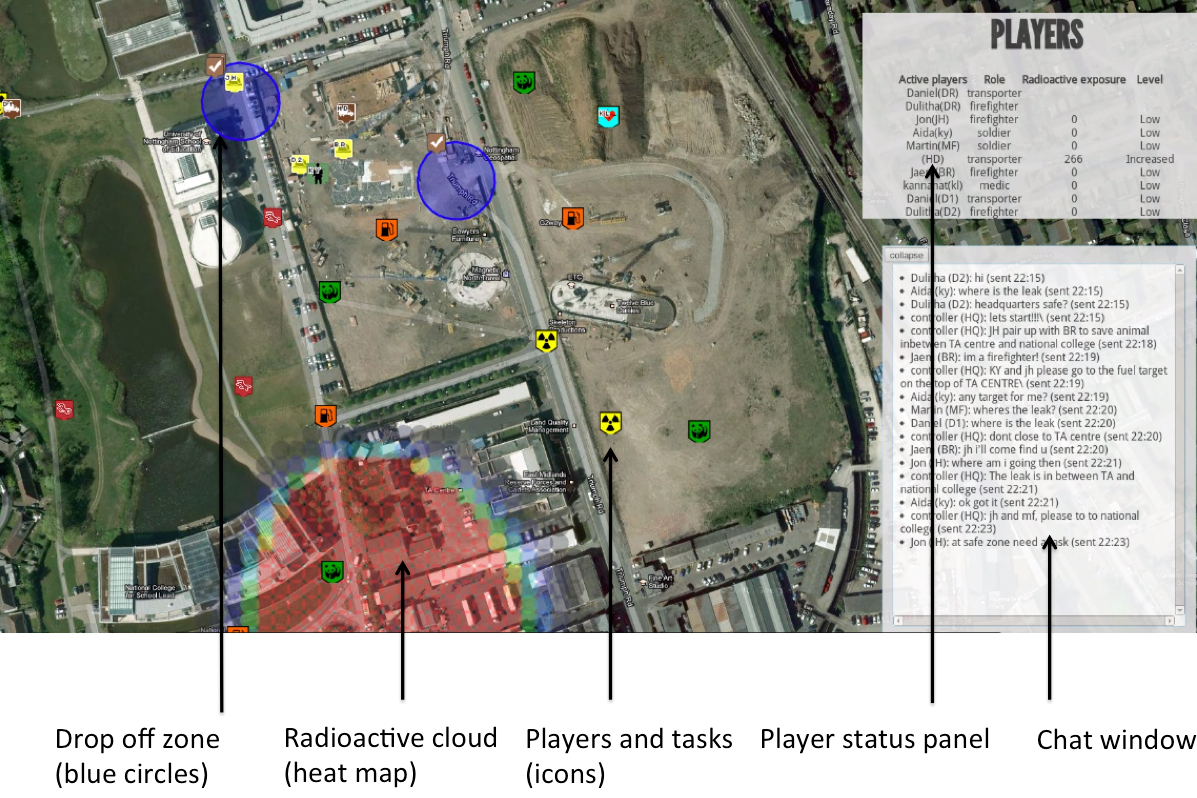
\includegraphics[width=1\textwidth]{img/study1/webinterface}
  \caption{The HQ interface}
  \label{fig:HQinterface}
\end{figure}

As you can see in the figure \ref{fig:HQinterface}, the majority space of the interface is occupied by a map-based presentation of the game status. Roles and locations of field responders are represented on the map as icons. The field responders can be uniquely identified by their initials shown on the icons. The target types and locations are also shown as icons on the map. Location and intensity of radioactivity is indicated by a heatmap. Health status (health value ranges from 0 to 100) of the field responders is displayed on the right-top panel. A chatbox is placed on right bottom for HQ to browse and send messages. The messaging system follows a broadcasting model. Everyone can send messages to one public channel, and the messages are visible to every play through the mobile and HQ interface.\\

Field responders are equipped with a mobile responder app providing them with sensing and awareness capabilities (figure \ref{fig:mobileResponderApp}). There are two tabs in the responder apps. The "map" tab displays a map showing locations of field responders and targets, which is similar to the map on HQ interface, except that the radioactvity is not shown. The radio level of players' current location is displayed as a Geiger counter reading (shown as a number on the top left of the screen ), which ranges from 0 to 100. Health status of the field responder is indicated by a health bar on the right side of the Geiger counter. The chatbox (similar to the one on HQ interface) is placed on the "Messages" tab for field player to receive and send messages.\\

% the mobile responder app
\begin{figure}[h]
  \centering
  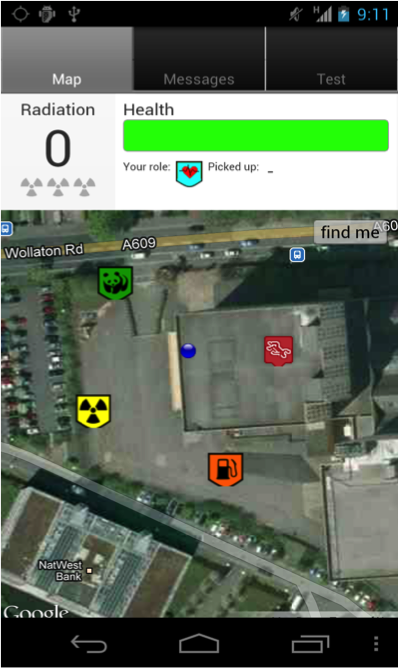
\includegraphics[width=0.5\textwidth]{img/study1/mobileinterface}
  \caption{The mobile responder app}
  \label{fig:mobileResponderApp}
\end{figure}

% move this to the study 1 chapter. 
 %The app shows a reading of radioactivity, their health level based on radioactive exposure, and a GPS-enabled map of the game area with the targets to be collected and the drop off zones for the targets. Icons according to responder roles that additionally have their initials on them can be used to identify individuals. Another tab reveals the messaging widget to broadcast messages to the other field responders, and to headquarters.\\

\section{Study Design}
% ====== checked from COOP, should be fine =======
We ran two AtomicOrchid Game sessions, with volunteers recruited from the local university. We describe participants, procedure, session configuration, and methods used to collect and analyse quantitative and qualitative data.\\

Study participants were recruited through posters and emails. A total of 18 participants were recruited; 7 participated in session A and 11 in session B. All participants were reimbursed with 15 pounds for 1.5 hours of study. In session 1, there are 1 HQ player and 6 field players. In session B, there are 8 field players and 3 field players. The majority of participants were students of the local university. Procedure. Upon arrival in the HQ (set up in a meeting room at the local university), participants were briefed and asked to consent to participate. Roles were randomly assigned to all participants (HQ/field responders: firefighter, medic, transporter, soldier). Field responders were provided with a smartphone; HQ coordinators with a laptop. Game rules and interfaces were introduced, and participants were assisted in setting up their phones and laptop clients. Field responders and HQ coordinators were given 5 minutes to discuss a common game strategy. All field responders were accompanied to the starting point within the designated game area, about 1 minute walk from headquarters.\\

Once field responders were ready to start, HQ sent a ``game start'' message. Gameplay commenced for 30 minutes. A ``Game over'' message by HQ concluded the game. Field responders returned to HQ for the post-game session. The post-game session consisted of a questionnaire aimed at collecting participants` feedback on (1) first impressions of the game; (2) usability of the system,and; (3) coordination issues in the game. A group interview was then conducted, before participants were debriefed and dismissed.\\

The size of the game area on the local university campus was 400 by 400 meters, without heavy traffic. The terrain of the game area includes grassland, a lake, buildings, roads, and footpaths and lawns. There are two drop off zones and 16 targets. The pilot study showed that this was a challenging, yet not too overwhelming number of targets to collect in a 30 min game session. There were four targets for each of the four target types. The pattern of cloud movement and expansion was the same for both game sessions.\\

We took a mixed methods approach to data collection and analysis. Five researchers with camcorders recorded the game play. One researcher recorded action in the HQ, and four other researchers each recorded a field responder team. In addition to video recordings, a semi-structured group interview was conducted aimed at eliciting important decision points, strategies and the overall decision-making process. We also developed a log file replay tool to help with data analysis of time stamped system logs that contain a complete record of the game play, including responders` GPS location, their health status and radioactive exposure, messages, cloud location, locations of target objects and task status. \\

\textbf{Data handling} Firstly, the log data (including remote messages) are handled by a digital replay system to reconstruct game play that can be triangulated with video data to support interaction analysis (Section \ref{sec:aprloghandling}). Secondly, to give an overview of how remote messages are used as a coordination resource, we used speech-act theory and the notion of adjacency pairs in linguistics to classify messages sent between and among responders and HQ (Section \ref{sec:aprmsg}). According to speech act theory, utterances in dialogues can be considered as speech acts from three dimensions. We were primarily concerned with the illocutionary dimension of speech acts. Searle`s classification of illocutionary acts \cite{Searle1976} is used to categorize messages in the communication system.\\

\textbf{Interaction analysis} We focus on the analysis of local field responders` interaction to unpack team coordination, including handling of messages sent by HQ. Video recordings of field action were catalogued to identify sequences (episodes) of interest (cf. \cite{Heath2010}). Key decision points in teaming and task allocation served to index the episodes. Interesting distinct units of interaction were transcribed and triangulated with log files of relevant game activity for deeper analysis that we present in this paper.\\

\section{Data analysis and results}
Here, we present findings from interaction analysis supported by message classification that reveal how team coordination was achieved. Overall, responders rescued 7 and 9 targets in session A and B respectively, out of 16 targets in total per session (Table \ref{tab:gameResults1}). Two players were incapacitated in session A, and 1 player was incapacitated in session B. 117 and 70 messages were sent in session A and B, respectively.\\

\begin{table}[h]
\footnotesize
\begin{tabular}{llll}
\multicolumn{1}{l|}{} & Saved targets & Incapacitated players & Remote messages \\ \hline
\multicolumn{1}{l|}{Session A} & 7 (out of 16) & 2                    & 117             \\ 
\multicolumn{1}{l|}{Session B} & 9 (out of 16) & 1                    & 70              \\ 
\end{tabular}
\caption{Overview of game results}
\label{tab:gameResults1}
\end{table}


In what follows, results of the message classification will be presented first, followed by detailed analysis of episodes.\\

% this is from COOP paper, need to adapt it for this writing 
%{An overview shows that directives from HQ are frequently not brought up locally. A further episode demonstrates how field responders instead draw on technological and embodied resources to achieve local coordination, without HQ involve- ment. Finally, two more examples illustrate how responders routinely employ messages as a resource to support situational awareness.\\ %}

\subsection{Results of message classification}
We used Searle`s classification of speech acts to categorize messages (Table \ref{tab:speechact}). The table x shows that the majority of massages are directives and assertives sent by HQ. The majority of messages from field responders are requests for information, team and tasks. In what follows, we present utility and examples for each category of speech acts, which in turn, provide an overview of remote coordination that heavily relies on the messaging system. \\

\begin{table}[h]
\footnotesize
\begin{tabular}{lllllp{5cm}l}
Speech acts  & \multicolumn{2}{l}{Session A} & \multicolumn{2}{l}{Session B} & \multicolumn{1}{c}{Example} & Total    \\ \hline
             & HQ            & FR            & HQ            & FR            &                                                                            &          \\ \hline
Directives   & 57            & 0             & 32            & 0             & JH pair p with BR to save animal in between TA centre and national college & 89(47)\% \\
Assertives   & 25            & 2             & 8             & 4             &                                                                        The leak around geospatial is bigger & 39(20)\% \\
Expressives  & 5             & 0             & 0             & 0             &                                                                           Good Job, JJ, TV and RL & 5(2\%)   \\
Declarations & 3             & 0             & 0             & 0             &                                                                           NOTICE - TEAM B: NS + TD & 3(1.6\%) \\
Commissives  & 0             & 4             & 0             & 4             &                                                                           ok got it & 8(4\%)   \\
Requests     & 8             & 6             & 0             & 19            &                                                                           wheres the leak? & 34(18\%) \\
Unclassified & \multicolumn{2}{c}{7}         & \multicolumn{2}{c}{2}         &                                                                            & 9(5\%)  
\end{tabular}
\caption{Speech act classification}
\label{tab:speechact}
\end{table}

\subsubsection{Directives}

Most messages in the category of directives are instructions sent by headquarter (HQ) players. The content of instructions can be related to two themes: task allocation and task execution. Therefore, we further categories the instructions into two categories: instructions for task allocation, and instructions for task execution. The purpose of task allocation instructions is to distribute plans to field teams and require them to execute it. Most instructions in this category follow a common pattern. Taking the following message as example:\\

\begin{quote}
\texttt{``HQ : JH1 pair up with BR to save animal inbetwen TA centre and national college''}\\
\end{quote}

The instruction sent from HQ consists of two parts: (1) Description of Teaming (who are involved) (2) Description of Location (Targets) to go.It is worth mentioning that HQ players use different strategies when they try to describe a location to field players. HQ players in session D frequently referred to landmark on the map in their description, while HQ in session C used simple directions (north, west, south east). For example:\\

\begin{quote}
\texttt{``HQ: TEAM A, can you head south to the radiation and animal targets? Instructions for task} execution''\\
\end{quote}

The purpose of task execution instructions is to help players execute their tasks after they have been assigned tasks. Most instructions in this category are related to radioactive cloud. To help field players avoid radioactive clouds, HQ players frequently send directions to field players or simply urge field players to move quicker. For example:

\begin{quote}
\texttt{``TEAM B you need to be quick''} \\
\end{quote}

\subsubsection{Assertives}

in this game, assertives provide plain information to recipients. Most assertives are sent by HQ because they have access to critical information - the cloud location. Followings are two examples of assertives:\\

\begin{quote}
\texttt{``the leak around nottingham geospatial is bigger''}\\
\end{quote}

\begin{quote}
\texttt{``HQ:There's another leak by the lake!''}\\
\end{quote}

Interaction analysis shows that assertives are important for field players maintain situational awareness. We will talk more about this shortly in the section \ref{sec:study1awareness}.\\

\subsubsection{Commssives, expressives and declarations}
We also identified a small number of commissives, expressives and declarations. Commissvies are field player`s response to an assertive or directive. It can be an acknowledgement of receiving a piece of information or commitment to execute a plan. (e.g. ``ok got it'', ``I am heading there'' ). Expressives are typically HQ`s congratulations to field players. (e.g. ``HQ:Good Job, JJ, TV and RL'' ) In session C, HQ players sometimes declare field players to be in a team (e.g. ``NOTICE - TEAM B: NS + TD''). The declarations help HQ to refer to a team easier.\\

\subsubsection{Requests and Adjacency pairs}\label{sec:adjpairs}
In linguistics, adjacency pair is a term to describe conversational turn taking. The pairs can be question->answer, inform -> acknowledge, offer->acceptance et al. For simplicity, we ignore the typology of adjacency pairs and treat all pairs as request-> response. Any utterance that expects a response is considered as a request. We found a number of requests sent from HQ and field players (14 in session A and 20 in session B). Those requests can be related to a number of themes (Table \ref{tab:requestThemes}).\\

\begin{table}[h]
\footnotesize
\begin{tabular}{l|ll}
                    & \multicolumn{1}{c}{Themes} & \multicolumn{1}{c}{Example}   \\ \hline
\multirow{3}{*}{FR} & Task assignment            & Anything for us to do?        \\
                    & Teaming                    & Firefighter with me for fuel? \\
                    & Cloud info                 & Wheres the leak?              \\ \hline
\multirow{2}{*}{HQ} & Player status              & Firefighter who is free now?  \\
                    & Acknowledgement request    & Firefighter, respond         
\end{tabular}
\caption{Themes of requests}
\label{tab:requestThemes}
\end{table}

In comparison, only a small number of adjacency pairs are found in both sessions (8 in C and 8 in D), which means not all requests are responded. (Table \ref{tab:adjpairs})



\begin{table}[h]
\footnotesize
\begin{tabular}{l|p{3cm}p{3cm}p{3cm}}
          & Total requests & HQ requests/ with no response & FR requests/ with no response \\ \hline
Session A & 14                                 & 8/7                                               & 6/1                                                \\
Session B & 20                                 & 1/0                                               & 19/14                                             
\end{tabular}
\caption{Adjacency pairs}
\label{tab:adjpairs}
\end{table}

It is also worth mentioning that field players didn`t send acknowledgements to directives from headquarter. Although we do not classify directives as a request which expect an answer, the headquarter players express their frustration for not having response to their instructions. A HQ player said in the group interview:\\
\begin{quote}
\texttt{``I guess they did not look at it, they could not respond it, we were like saying ``where are you, respond'', but they did not respond. I guess they are busy seeing themselves and the targets''}
\end{quote}

A field players also commented on the issue:\\

\begin{quote}
\texttt{``I almost would not use the communication system because I was too focused on trying to save the targets.''}
\end{quote}

\begin{quote}
\texttt{``Sometimes I check whether the radiation is close to us, but mostly the communication is between us (local team members)''}
\end{quote}

\subsubsection{Summary}
To sum up, the majority of messages are assertives and directives from HQ. Directives are instructions sent by HQs as their attempts to guide/control task planning and execution of the team, while the assertives are mainly informational content about status of the danger zone (i.e. the cloud). Small number of commssives, expressives and declarations are also found in the messages. Both HQ and field responders send requests for various purpose (e.g. request for task, teammate, cloud status, confirmations). Based on analysis of adjacency pair, responses to the requests are poor, which align with the player's comments about their experience of using the message system.

\subsection{Responding to directives from HQ}\label{sec:study1directives}
% TODO introduce episode 2 in my part as a simple unproblematice case here!!

We examine how field responders deal with messages from HQ that attempt to allocate tasks and manage task execution (i.e., directives). Classification of messages showed that directives were exclusively sent by HQ, and that they were the most frequent kind of message (Table \ref{tab:speechact}). Overall, out of the 43 directives HQ sent for task allocation, the recipient field responders brought up only 15 messages in conversation in the team. The instances in which task allocation messages were addressed reveal the handling and value of HQ directives in the local coordination. Firstly, out of the 15 task allocation messages responders talked about, they decided to ignore the instructions only once. The re- sponders ignored instructions because they were engaged in another task that they did not want to abandon. Secondly, four HQ instructions to rescue a certain target coincided with the same plan that had already been made locally by the respond- ers. In 10 cases, field responders chose to follow the instructions. However, due to confusion and misunderstanding they failed to follow them correctly six times. In fact, only 2 instances of directives from the HQ led to task completion. For the remaining 14 saved targets, field responders had locally allocated the tasks without HQ.\\

% ===== insert the diagram from the JCSCW paper not COOP
\begin{figure}[h]
  \centering
  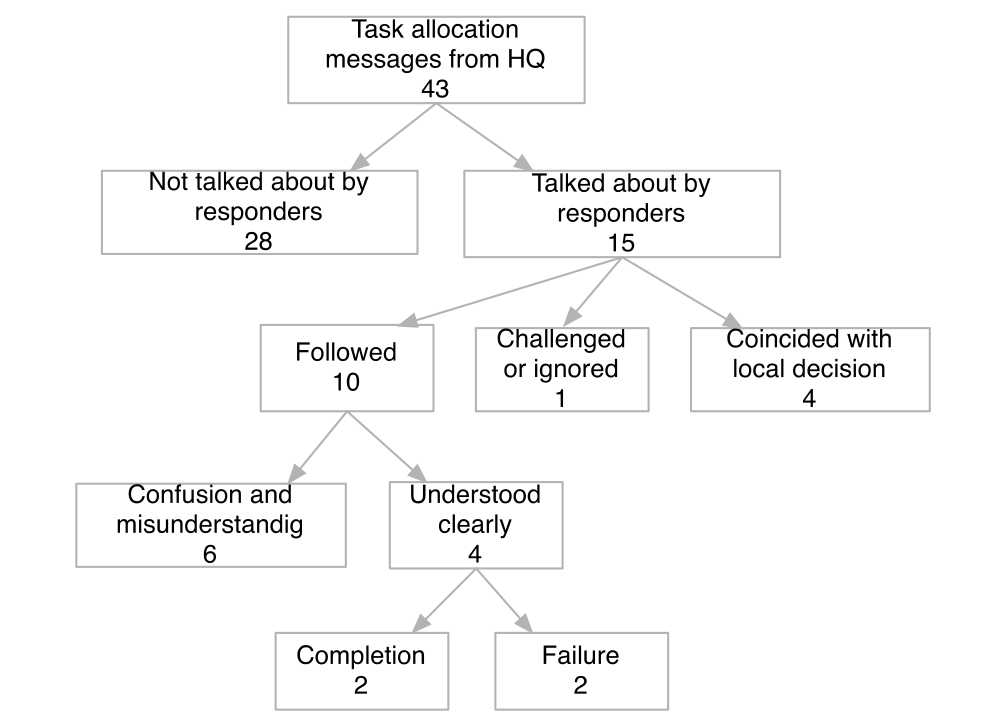
\includegraphics[width=1\textwidth]{img/study1/instructions}
  \caption{How responders addressed task allocation messages from HQ.}
  \label{fig:instructions}
\end{figure}

Directives index (attempted) the instances of remote coordination of field responders by HQ. The observed response to messages is critical to understanding relationships between local and remote coordination. The following episode depicts a team of three on their way to pick up fuel. Their path is blocked by radiation. Without a team, firefighter JH (on the left) has just joined soldier KY (on the right), and firefighter D2 who have just been allocated a task in a message by HQ. (Figure \ref{fig:study1ep11})\\

\begin{figure}[h]
  \centering
  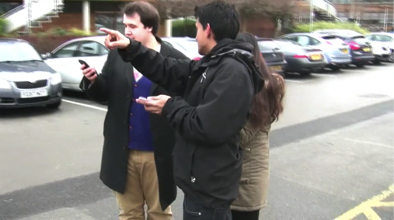
\includegraphics[width=1\textwidth]{img/study1/ep1/ep11}
  \caption{episode 1.1, JH (Behind Left), D2 (Middle Front), KY (Right behind)}
  \label{fig:study1ep11}
\end{figure}


\noindent \texttt{\textbf{Episode 1.1}\\
\textbf{KY:} ((reading out message)) KY and D2, please walk fast to the junction and quickly return back ((laughs))\\
\textbf{D2:} Oh is that what we have to do? Ok so we have to run to (2.0) We need to work out where we have to run to first and then get (.) get it back. Which junction is that? If you run to the next (0.5) thing ((points)), and then come back (1.0) that would work (1.0) is it safer to go around?\\
}


\begin{figure}[h]
  \centering
  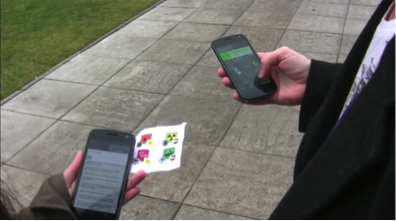
\includegraphics[width=1\textwidth]{img/study1/ep1/ep12}
  \caption{episode 1.1, KY (Left) , MF (Right) holding mobile phones}
  \label{fig:study1ep12}
\end{figure}


\noindent\texttt{\emph{[The team tries to go around the cloud but is stopped by radiation, realising their target is in the cloud. Meanwhile, D2 has left due to increased exposure.]\\}
\textbf{KY:} So we have to run! [through the radiation] \\
\textbf{JH:} Do we have to run through the (.) through the radiation? ((looking at map)) (Figure \ref{fig:study1ep12})\\
\textbf{KY:} Yah this is what the headquarters told us to do ((looking at messages)) \\
\textbf{JH:} I have a terrible feeling thats gonna kill us.\\
\textbf{KY:} But its gonna be meaningful ((laughs))\\
\textbf{JH:} We go around this corner, if it gets to half [referring to health] we should probably start running back.\\
\emph{ [KY JH begin running into the cloud] } (Figure \ref{fig:study1ep13})
}

\begin{figure}[ht]
\centering
\begin{minipage}[b]{0.45\linewidth}
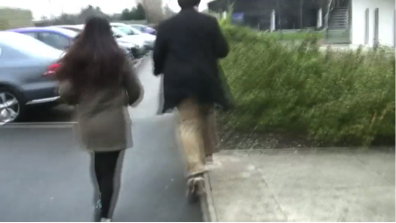
\includegraphics[width=1\textwidth]{img/study1/ep1/ep13}
\caption{episode 1.1, KY,MF running into cloud}
\label{fig:study1ep13}
\end{minipage}
\quad
\begin{minipage}[b]{0.45\linewidth}
 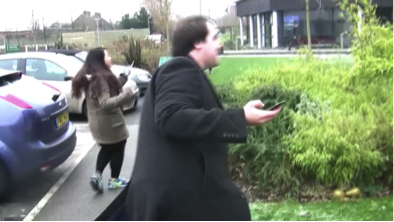
\includegraphics[width=1\textwidth]{img/study1/ep1/ep14}
\caption{episode 1.1, KY,MF escaping from the cloud}
\label{fig:study1ep14}
\end{minipage}
\end{figure}
\noindent\texttt{\textbf{KY:} ((yells)) OH OH! It`s a hundred! [refers to radiation level]\\
\textbf{JH:} We are basically in the middle of it! We are basically in the middle of it!\\
\textbf{KY:} ((shouts)) I`m going back? Get the fuel first! Get the fuel first! Oh no! \\
\textbf{JH:} We are not prepared for that! I blame our HQ.\\
\emph{ [They turn around and run back out of the cloud without the fuel.] }(Figure \ref{fig:study1ep14})\\
}



This episode begins with a message by HQ attempting to help give directions to the target. D2`s response to the message is hesitant (is that what we should do?). His following question (which junction is that?) suggests the referent in HQ`s message is not understood. They attempt to go around the radiation. They realise their target is in the cloud. They refer back to the message to support their intent to go into the cloud to attempt to save the target (Yah this is what the headquarters told us to do). Having run into the cloud, they refer to the Geiger counter and realise the exposure is too high. Meanwhile, their health is decreasing rapidly. They abandon the task and flee to safety, whilst JH expresses his frustration (We are not prepared for that. I blame our HQ.).\\

First, the episode shows that geospatial referencing in messages can be problematic. It is unclear to the responders which junction HQ is referencing (and the responders do not ask for clarification), so they revise the route themselves. At the same time, they draw on the messages to justify their entering of the cloud. It does not occur to the responders that HQ allocated the task at an earlier time, before the cloud had covered the target. HQ does not update the responders on the increased danger, or revise their earlier task allocation. When the responder team fails to complete the task, they place blame instead of thinking self-critically.\\



\subsection{Local coordination without HQ}\label{sec:s1localcoordination}
As presented, field responders predominantly coordinated teaming and task allocation without HQ instructions. Recall that 14 targets are saved without HQ's instructions, versus only 2 targets that are saved with HQ's instructions. The following episode illustrates how field responders achieve coordination of teaming and task allocation locally. We join the action as BR and another responder are waiting at the drop-off zone without a compatible teammate, as MF and his teammate join and drop-off their target.\\

\begin{figure}[ht]
\centering
\begin{minipage}[b]{0.45\linewidth}
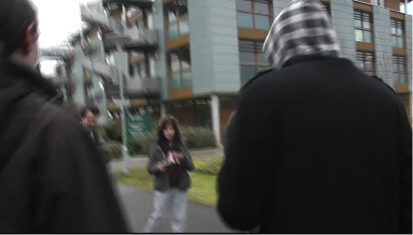
\includegraphics[width=1\textwidth]{img/study1/ep2/ep21}
\caption{episode 1.2, MF (right), BR (middle)}
\label{fig:study2ep21}
\end{minipage}
\quad
\begin{minipage}[b]{0.45\linewidth}
 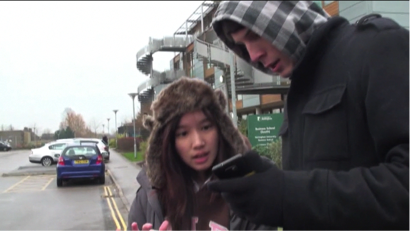
\includegraphics[width=1\textwidth]{img/study1/ep2/ep22}
\caption{episode 1.2, MF (right), BR(left)}
\label{fig:study2ep22}
\end{minipage}
\end{figure}

\noindent\texttt{\textbf{Episode 1.2}\\
\emph{[MF (on the right) and teammate walking towards BR (center)]\\}
\textbf{BR:} Any soldiers?\\
\textbf{MF:} I am soldier yeah.\\
\textbf{BR:} Would you like to pair with me? (2.0) to rescue a fuel?\\
\textbf{MF:} what are you after?\\
\textbf{BR:} I am a firefighter.\\
\textbf{MF:} Soldier and firefighter is fuel isn`t it?\\
\textbf{BR:} yeah.\\
\textbf{MF:} What can we get? (2.0) ((looks at screen)) this one in the center? ((points at screen))\\
\textbf{BR:} ((glances MF`s screen)) I think there are two people (the team D2,KY) going for that. I think we should go for this one ((points at screen)).\\
\textbf{MF:} We are going to get killed ((both laugh)).\\
\emph{[The team begins walking to target.]}\\
}

At the beginning of the episode, MF met BR, who was waiting at the drop-off zone without a compatible teammate. BR requested to team up with MF (``Would you like to pair with me? (2.0) to rescue a fuel?'') after MF identified himself as a soldier. BR and MF can then be observed sharing the screen of his device and using the map to identify potential targets (fuels) (Figure \ref{fig:study2ep22}). They realise one of fuel targets is already being pursued by another team. They agree on another target fuel to pursue. Note that messages do not play a role in this episode. It exemplifies how teaming and task allocation are achieved locally, without consulting HQ. \\

The next episode is a follow-up episode, which demonstrates how two teams resolve the conflict when they approach a same target.\\

\begin{figure}[h]
  \centering
  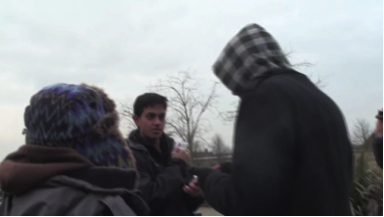
\includegraphics[width=1\textwidth]{img/study1/ep5/ep51}
  \caption{episode 1.3, MF(right), BR(left) met with D2(middle)}
  \label{fig:intructions}
\end{figure}

\noindent\texttt{\textbf{Episode 1.3}\\
\textbf{D2:} we are told to get this fuel (target 1) from HQ.((pointing to screen))\\
\textbf{MF:} you are going to the fuel (target 1) we are aiming for, we thought you are going for this one (target 2).\\
\textbf{D2:} we were until we got a message saying not to. \\
\textbf{MF:} you get that one (target 1), we get that one (target 2).((pointing to the two target locations))\\
\textbf{D2:} if you want get that one (target 2). It is somewhere in the building.\\
\emph{[The two teams split, proceed with the new target allocations]}\\}

At the beginning of this episode, the team (BR, MF) has decided to pursue (see episode 1.2) a target other than the one pursued by team D2, KY. However, instructed by HQ, MF and KY changed their target and met BR and MF on the way. The two teams then began to show their intended targets to each other. After they find they are heading to a same target, MF suggest a new allocation of tasks (``you get that one, we get that one.''). D2 then offered some information about the target location to the team MF,BR (``if you want get that one. It is somewhere in the building.''), suggesting he agreed with the new task allocations proposed by MF. \\

The two previous episodes show that how teaming and task allocation are achieved in a ``ad-hoc'' manner. By using the word ``ad hoc'', we stress the the actions of field responders are typically not planned ahead adequately. The players often exchange information through conversations when co-located, and their plans are ready to be changed when new information is acquired. Take episode x as an example, while BR was waiting at the drop-off zone, she requested to team up with MF who happened to pass by. MF agreed to team up and then decided to aim for an available target that have not been aimed by others. In episode y, the two teams quickly came up with new task allocations when they found they were actually heading to the same targets . In the interview at the end of study, field responders also confirmed their ``ad-hoc'' behaviour in the interview:\\

\begin{quote}
\texttt{``Just save the closest target then just pair up and go to the other one'' }
\end{quote}

\begin{quote}
\texttt{``We just check, with that group, which target we can get. We see on the map to find the closet one we can get.''}
\end{quote}

% Add an episode from my part how the field responder resolve conflicts, suggest it is opportunistic. 



\subsection{Remote messages as a resource of situational awareness} \label{sec:study1awareness}
In the AtomicOrchid game, field responders need to be aware of what other responders are doing, where the `danger zone' is (the cloud), and where it is likely to move. Awareness of each other`s actions helps responders avoid conflicts in planning, while awareness of the danger zone is essential to survive. The following episode illustrates how responders use remote messages as a resource to gain situational awareness.\\

The episode takes place towards the end of game session B. The radioactive cloud has grown so much that navigation in the game area becomes increasingly difficult. MF is with a group of five responders, two of which are carrying an animal. The cloud is blocking their way towards the drop off zone; they stop.\\

\begin{figure}[h]
  \centering
  
\includegraphics[width=1\textwidth]{img/study1/ep3/ep31}
  \caption{episode 1.4, MF pointing to a building}
  \label{fig:study1ep31}
\end{figure}

\noindent
\texttt{\textbf{Episode 1.4}\\
\textbf{MF:} ((reads message from HQ out loud)) There is another leak around Geospatial. (1.0) Which is Ah: so there`s a leak sprung up there. ((points)) Geospatial is like (.) that building right there. They say there is another leak. We should go all the way round (0.5) to the top left one, I think. (Figure \ref{fig:study1ep31})\\
}

MF brings up HQ`s message of the new leak, and suggests a route around the new cloud. The group ends up following MF`s route suggestion as a result. News of the new cloud, provided by HQ, enables the group to change their route to avoid danger. We commonly observed responders sharing information that provides situational awareness through face-to-face conversation. In the previous example, MF shared the message with a group of responders he was with already. The following example takes place between D2 and his teammate, as they are approached by JH, who is currently without teammate.\\

\begin{figure}[h]
  \centering
  
\includegraphics[width=1\textwidth]{img/study1/ep4/ep41}
  \caption{episode 1.5, JH(left) met team D2(male, middle) and KY(female, right)}
  \label{fig:study1ep41}
\end{figure}

\noindent
\texttt{\textbf{Episode 1.5}\\
\textbf{JH:} Where are you guys heading? \\
\textbf{D2:} To get the fuel.\\
\textbf{JH:} Okay. The closest one to you? \\
\textbf{D2:} I believe so.\\
\textbf{JH:} Ya okay cuz I think the leak is somewhere near the other one and the army. [referring to building]\ref(Figure \ref{fig:study1ep41})\\
\textbf{D2:} Oh (.) which one?\\
\textbf{JH:} They sent a message saying its between territorial army center. 
\textbf{D2:} We are trying to get the one here ((points)).\\
\textbf{JH:} The closest one. Okay.\\
}


Making use of the map as he approaches them, JH asks the others to clarify which fuel they intend to pursue (the closest one to you?). He proceeds to inform the team that the ``leak is somewhere near the other one''. D2`s response (Oh, which one?) suggests they did not know this. In turn, JH elaborates on the location of the cloud, using an anonymous ``they'' to refer to the source of his information. ``They'' is likely to refer to HQ as they previously sent a message with the information of the cloud`s location. Conversational sharing of important information was a common resource responders employed to achieve and maintain situational awareness. However, requests for information in the messages channel were regularly not reciprocated with a response: out of 14 requests in session A, 8 were not responded upon; and in session B, 14 out of 20 requests were not responded upon (Table \ref{tab:adjpairs}).\\

\section{Discussion}
This section will present broader concerns emerged from the game for the design of HAC systems that support task planning and team coordination.\\

\subsection{Division of labour}\label{sec:study1dlabour}
Firstly, the HQ plays an important role in providing situational awareness to the whole team. As the game mechanic provides the HQ exclusive access to location of radioactivity, the HQ managed to provide informational messages about the radioactivity to field players. Field players are able to pick up the information and spread it to other field responders through face-to-face conversations (Episode 1.2). Although HQ attempted to organise task allocations directly (through directives), their attempts are often problematic.  Although the field responders did not get too much planning support from HQ, they naturally organise themselves into small teams and carry out tasks. As shown in episode 1.4 and 1.5,  face-to-face conversation is vital for task and team organisation. We observed that co-located team members collectively make sense of the remote messages and game status shown on mobile screen. The decisions such as choices of team, targets and routes are  predominately made through local conversations.\\

The pattern of division of labour between field responders and HQ indicates the weak role of HQ in terms of task planning. The responder's choices of teams and targets seem to follow an ``ad-hoc'' manner as they heavily rely on face-to-face conversation , which can only happen when players are co-located. Despite some disruptions from communication channel (misunderstanding and confusions), field players seem to be able to find team-mates and avoid conflicts in their plans (e.g. avoid pursuing the same target) through local coordination. 




\subsection{Breakdown of remote coordination}\label{sec:study1breakdown}
The observed division of labour (Section \ref{sec:study1dlabour}) highlights heavy reliance on the local coordination. To some extent, the heavy reliance on the ``add-hoc'' local coordination can partly be a result of the lack of remote coordination support. In other words, local coordination become important when system support for remote coordination is problematic. In a co-located setting, players can naturally make their actions observable and accountable to each other through conversations, body languages, gestures , screen sharing et al, and organise coordination activities reflexively. However, in the remote setting, the natural accountability of their activities become opaque. The game probe provides a set of functionalities supporting remote coordination, including GPS/map sharing, broadcasting. We have observed players utilise the functionalities to make sense of other team members' actions (see section \ref{sec:s1localcoordination}) and act accordingly. However, coordination with remote players is still overall problematic which can be evidenced by lack of response and acknowledgements to requests in the messaging channel (Section \ref{sec:adjpairs}); Misunderstanding and confusions observed when field responders try to follow the directives from HQ (Section \ref{sec:study1directives}).\\

We suggest the future planning support should properly support remote coordination in a way that facilitate accountability among distributed team members. The section x discuss some detailed requirements of remote coordination support drawn from the field observations. The next section expands on the design requirements that can enhance remote coordination in a way that supports natural accountability of human activities.\\

%{ The natural social order that employed by the team members to make sense of the task environment. Players are observed to constantly revealing to others their action and plans via face to face conversation. CSCW concern that Geo-spatial distribution distributed  hinders team member's attempt maintain accountability . The lack of response in the communication channel shows that. The form of communication in this study appears to be unable to support the team member's accountability. The missing of remote coordination and the weak role of HQ in the planning activities may indicate communication breakdown, which can also be confirmed by a number of observations of understanding and confusions in the communication channel (see x.x.x).\\From this perspective, the domination of local coordination . Some of the reasons? %}

\subsection{Implications on computational support}
%[connect to situated planning by Lucy suchman] it is a kind of situated action. \\
% It is important that we do not treat human plan in an inferir way. They are about to leverage all the resources avalible to make deblibration on their actions. Supporting them a plan will be the same as augmenting their resources. How the team organsie their activities around this resouces can be makde subjuct of study. and study about that can lead to interaction design that support situation

To some extent, the observation of ``ad-hoc'' local coordination is aligned with the view of situated actions. As a whole team, players form and disband teams without holistic plans prior to their actions. Players are observed to have conversations about their status, on-going activities when they meet up. Local decisions for next move are often made during the conversation.  Information from mobile interface (e.g. player locations, radiation readings and messages) are often brought to conversions as resources for their situated actions. 

The lack of plans may indicate the lack of optimisation of team task allocation. The multi-agent coordination algorithms (e.g. \cite{Ramchurn2010}) appears to be about to support the team by producing computationally optimised plans for responder teams. However, design of the planning support may not be straightforward. \\

Firstly, there is a danger to impose an inappropriate ``work model'' (assumed by agent support) on the human team. The studies of CSCW systems \cite{Bowers1994} raise a concern that the work model held by the technological system sometimes comes into tension with the natural human workflow achieved through methods internal to the work. For example, current division of labour between HQ and field responder suggest that HQ plays a supportive role (providing situational awareness). However, a centralized coordination algorithm may need to coordinate the whole team, requiring every players to follow top-down instructions to reach global optimum of resource allocation. In that case, the role of control room may need to change and it is unknown whether the change will disrupt or support human workflow. \\

Apart from disruption of human workflow, there is also danger for the supporting system to impose a planning on human teams. Suchman suggests that human's situated action should not be simply treated as a inferior version of scientific planning model. Following the view of situated actions, supporting human's actions are not as simple as providing an optimised plan to execute. A plan for human teams is only one of the resources that human can utilize for their deliberation on their actions. Therefore, the role for the system is to provide plans (as an extra resource) in a way that support human's situated actions. \\

Adopting the view of human agent interaction, we can treat a plan support system as a teamwork agent.  Achieving mutual intelligibility between the agent and the human team can also be a major design challenge.  As plans from the agent is only a representation of possible actions and effects based on simulations. How the responders make use of plans can be highly dependent on mutual intelligibility. For example, it would be problematic if globally optimised choices conflict with the ``ad-hoc'' choices that are obvious for human field responders. We can not assume either the agent or human choice will be always correct, perhaps neither of them can take an authoritative role. Therefore, we need to carefully design the interaction between human and agent to ensure that they maintain mutual intelligibility so that informed collective decisions can be reached.  \\

%which is often the main concern of multi-agent coordination algorithm. However, the dominance of ``ad-hoc'' local coordination indicates the absence of the notion of resource optimisation. In a sense, it opens opportunity for computational support, but it also highlights some potential challenges for such support system. 


\section{Design Requirements}\label{sec:study1requirements}
Drawn on the problems observed in remote coordination (Section \ref{sec:study1breakdown}), we now discuss the design requirements that enhances remote coordination. The embodied game probe embedded responders in a challenging setting. They needed to communicate effectively to make time critical decisions on teaming and task allocation, both locally in the field as well as remotely through messaging. Field responders physically engage and navigate the environment to perform tasks while maintaining awareness of risk and danger. The data reveals multiple challenges for team coordination involving communication and decision-making. \\

\textbf{Sharing of local decision-making} The study showed that teaming and task allocation were predominantly organised locally among field responders, in an ``ad-hoc'' manner, on-the-fly fashion. Despite the fact that HQ attempted to coordinate task allocation remotely, few of these directives were brought to conversation locally. Only 2 out of 16 tasks that field responders completed were remotely allocated by HQ (Figure \ref{fig:instructions}). Although players are able to smoothly conduct local coordination, the local coordination heavily relies on and limited by the face-to-face conversations, which means some conflicts of planning can only be found and resolved when players meet each other (e.g. episode 1.3). Therefore, the local decision-makings can benefit from a shared picture of team-wide planning decisions. We thus argue that local decision-making needs to integrate capabilities to enable team-wide sharing of the local decisions.\\

\textbf{Coordinate resources} While field responders made decisions on teaming and task allocation in a seemingly ad hoc fashion, game data reveals how field responders draw on resources to achieve situational awareness in order to coordinate successfully. A common understanding of the location and movement of the radiation cloud was achieved by sharing information from game messages verbally in a local group. Face-to-face talk was an essential resource for relaying information from the Mobile Responder App to teammates, such as radioactive exposure, others` whereabouts, task status, and other monitoring of the broadcast messages. Future planning support systems need to take into account that such coordinate resources are likely to be comprised of digital as well as embodied human resources. \\

\textbf{Geospatial referencing} The results show that geospatial referencing was problematic in various ways, particularly in directive messages sent to the field players. Participants had different levels of knowledge of the campus, which made understanding of landmark references uncertain. Some participants also struggled with making sense of north/south/east/west directions in relation to their current position and orientation. To deal with misunderstandings, players had to ask for clarification via messages or spend valuable time discussing the reference locally in order to understand it. Consistent with the findings of Toups et al. (2009), designers need to think carefully about how the presentation layer of HAC systems may be augmented with information that facilitates geospatial referencing (e.g., grids, labelling etc.) to facilitate human in addition to machine readability. Freshness of messages. Problems arose from erroneous instructions or otherwise out-dated messages sent to field responders. In one case HQ sent a message in which two players with non-compatible roles were instructed to team up. This was particularly costly, as the players attempted to team up, and lost valuable time until they realised the game mechanics barred them from forming a team.\\

\textbf{Freshness of messages} As demonstrated in one of the episodes, reading out-dated messages in a dynamically changing environment can contribute to responders taking dangerous actions that they believe to be safe, because they do not realise that the infor- mation is out-dated. However, in most cases, recipients managed to identify temporally irrelevant messages, and thus avoided following them.\\

To reduce confusion about message freshness, HAC systems should address these issues at the UI level, both for responders and for HQ. Develop functionality to flag messages as out-dated or retract incorrect messages. Up-to-date messages are particularly valuable. Thus, our findings support the use of fresh social media as a source of information for disaster response, despite problems that can arise with validation, because crowdsourced information will in many cases provide better coverage than official sources.\\

\textbf{Acknowledgement of messages} In most cases, field responders did not acknowledge or respond to messages sent by the HQ. This was particularly problematic for directives (task allocation), as task status and field responder compliance often had to be inferred by observing their location updates on the map. This consumed HQ attention, with negative impact on HQ`s overall work on state assessment and task planning. Observations in the field suggest that the physical demands (e.g., co-located team movement through terrain at speed) and cognitive demands to maintain situational awareness (e.g., monitoring of radioactivity and messages) are likely factors that explain lack of acknowledgement.\\

As a result, user interfaces that enable and encourage field responders to quickly acknowledge HQ messages, with minimum cognitive load, should be consid- ered for messaging in HAC systems in such high demand settings. For effective team coordination in disaster response, interface and workflow designs need to factor in cognitive load and task demands for effective information distribution.\\


\section{Summary}
The objective of this study is to unpack how human teams coordinate in the time and space constrained task setting. In particular, we focussed on a scenario in which responders coordinate role-based teaming and spatially distributed task allocation and execution using a real-time location and messaging system.\\

We presented the design and study of the AtomicOrchid ame as a mixed-reality game probe to investigate challenges for team coordination in a set- ting in which participants experience both physical strain through bodily activity, and cognitive challenge through time pressure and task complexity. We eschew high-fidelity simulations in favour of mixed-reality game probes as a platform for investigation of concomitant socio-technical issues: handling of mobile devices to communicate and maintain situational awareness (messaging, sensing, interaction, and display) intersect with face-to-face interaction, whilst the physio-cognitive challenges created through game mechanics and environment induce stress. We created a setting that allows exploring requirements to support team coordination of relevance to time-critical coordination domains such as real disaster response.\\

Findings from interaction analysis of field observations, triangulated with log files, reveal how field responders achieved coordination by drawing on local face-to-face conversation with fellow responders, and situational information provided by the interactive map, the Geiger counter, and the messages sent by HQ. Drawing on these findings, we generated requirements for supporting team coordination, emphasising the roles of local coordination, decision-making resources, geospatial referencing and message handling. These requirements inform future work on building planning support system by emphasising the role of human interaction in team coordination in time-critical settings.\\

%************************************************
\chapter{AtomicOrchid Study 2: The Human On-the-loop Design}\label{ch:studytwo} % $\mathbb{ZNR}$
%************************************************
This chapter presents the second iteration of AtomicOrchid field trials. In this study, a planning agent is integrated into the system by following a Human On-the-loop interaction design, in which the HQs only monitor and occasionally intervene the planning agent. The purpose of the trials is to investigate socio-technical issues related to human agent interaction. Interaction analysis is conducted to examine log data and field observations unfolding how human agent interaction plays out, which in turn, revealing the process by which players interpret and negotiate the agent guidance as well as how these are intertwined with social dynamics of the teams.

\section{Introduction}\label{sec:studytwointroduction}
Task planning in teams can be complicated by both spatial and temporal constraints, particularly in time-critical task domains such as disaster response (DR). In a DR setting, responder teams have to coordinate sparse resources and personnel to prioritize geographically distributed tasks, forming and disbanding teams dynamically to carry out DR operations \cite{Chen2005}. Multi-agent researchers have devised a number of agent coordination algorithm to coordinate task allocations for multi-agent systems, which can be adapted to support planning activities of DR teams. \\

However, these algorithms typically model humans as computational agents with respective capabilities, for example to dynamically allocate teams of agents to tasks in order to maximise an objective (e.g., number of lives saved), taking into account other aspects of the real world (environment, infrastructures, victims, etc.) \cite{Ramchurn2010a}. Therefore, the quality of the planning results can be constrained by limited assumptions of human behaviour (e.g., human psychosocial characteristics, movement, and learning ability) and real world environment \cite{Armenakis2012}. These limitations highlight importance of human input in the planning process. Thus, we argue that effective collaboration between human and agent is required to produce and execute high quality plans in the disaster setting. . \\

In order to support effective Human agent collaboration, two patterns of interaction design (Human On-the-loop and In-the-loop) are presented in section \ref{sec:patterns}. In this study, the planning agent is integrated into the AtomicOrchid system with a straightforward Human On-the-loop design (Figure \ref{fig:study2OnTheLoop}). This design assumes minimal Headquarter intervention, that is, the agent can directly interact with field responders to generate and implement plans without constant involvement of HQ. The interaction design is aimed to facilitate a pattern of division of labour, in which a planning agent routinely assigns tasks to distributed responder teams, while human coordinators (the HQ) monitor and support the task execution by responding to arising contingencies. The agent is designed in a way to take into account simple human feedback, i.e., a field responder can either reject or accept their task assignment. The agent will consider the feedback for the next iteration of task assignment.\\

\begin{figure}[h]
  \centering
  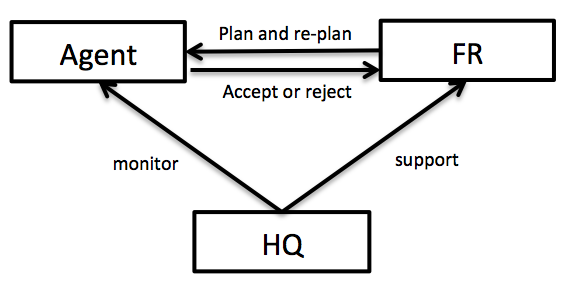
\includegraphics[width=0.7\textwidth]{img/approach/OnTheLoop}
  \caption{On-the-loop interaction design}
  \label{fig:study2OnTheLoop}
\end{figure}

This study uses the agent integrated version of AtomicOrchid as a probe to unfold socio-technical issues in human-agent interaction, with focus on the implications of the Human On-the-loop design on human team performance. More specifically, this chapter addresses the following research questions on how agent guidance affects the social organisation of team performance:\\

\begin{enumerate}
\item How do human teams respond to being instructed by an agent, particularly on switching teams and tasks?\\
\item The planning agent makes decisions based on limited assumptions about human behaviour, but what are the hidden costs of human behaviour that the agent does not take into account?\\
\end{enumerate}

Findings from the study highlight the social processes in which members interpret, negotiate, and manage the agent guidance within the social dynamics of teams. We discuss the division of labour between humans and teams; the hidden costs of instructions that suggest team reformation and interrupt on-going tasks. We conclude the paper with a number of emerging interaction design recommendations to consider when building planning support systems for human teams, which emphasise the need for common ground between humans and the agent, facilitate accountability between team members, and balance responsibilities between humans and the planning agent appropriately.\\


% ===== from CTS need adaptation =====
%We present a field trial of how instructions from an intelligent planning agent are dealt with by distributed human teams, in a time-critical task setting created through a mixed-reality game. We conduct interaction analysis to examine video recorded field observations and game log data. The findings highlight the social process by which players interpret and negotiate the agent guidance as well as how these are intertwined with social dynamics of the teams. The insights can be used to develop an understanding of interactional issues around automated team instructions and inform the design of human-centred planning support systems. \\

%Task planning in teams can be complicated by both spatial and temporal constraints, particularly in time-critical task domains such as disaster response (DR). In a DR setting, responder teams have to coordinate sparse resources and personnel to prioritize geographically distributed tasks, forming and disbanding teams dynamically to carry out DR operations [4]. For example, teams of fire fighters and medics are required to extinguish a fire and to provide first aid, while teams of soldiers and transporters may be needed to clear rubble. These teams, in turn, may need to disband and reform dynamically to perform new tasks and to adapt their planning to uncertainties in real time. Whilst an `optimal' plan of team formation and task allocation may help minimise loss of lives and properties, making optimal plans in real time can be complicated and time-consuming due to large numbers of incidents and responders. To address such coordination challenges, multi-agent research has developed a number of smart coalition formation algorithms to computationally support planning in time-critical task settings [3,16]. These algorithms typically model humans as computational agents with respective capabilities, for example to dynamically allocate teams of agents to tasks in order to maximise an objective (e.g., number of lives saved), taking into account other aspects of the real world (environment, infrastructures, victims, etc.) [14]. \\

%However, most of these smart algorithms are based on limited assumptions about human behaviour (e.g., human psychosocial characteristics, movement, and learning ability) [18], and have only been evaluated in computational simulations. In our work, we investigate agent-based planning support in the real world. Specifically, we study the social implications of the division of labour between agents and real human teams. In more detail, while coalition formation assumes leaving and joining new teams as an unproblematic process, we study in depth the social, interactional consequences of agent-based instructions that require team formation. For example, Personal preference and social norms may imply that dynamic team formations have a hidden social cost that may impact team performance. \\

%We present AtomicOrchid, a mixed-reality game probe of the ways in which human teams respond to agent guidance. The probe is designed to create a socio-technical setting in which distributed teams and a planning agent work collectively to save locally dispersed targets on the ground. The planning agent runs a coalition formation algorithm to help allocate tasks optimally to the teams. Our analysis reveals social implications of agent support for human teams. In turn, implications for interaction design are discussed that may improve team performance. More specifically, this paper addresses the following research questions on how agent guidance affects the social organisation of team performance:\\

%How does division of labour play out between humans and agents and how should it be scaffolded by design? 
%How do human teams respond to being instructed by an agent, particularly on joining and leaving teams?
%The planning agent makes decisions based on limited assumptions about human behaviour, but what are the hidden costs of human behaviour that %the agent does not take into account?\\

%Findings from the study highlight the social processes in which members interpret, negotiate, and manage the agent guidance within the social dynamics of teams. We discuss the division of labour between humans and teams; the hidden costs of instructions that suggest team reformation and interrupt on-going tasks. We conclude the paper with a number of emerging interaction design recommendations to consider when building agent-based support systems for human teams, which emphasise the need for common ground between humans and the agent, facilitate accountability between team members, and balance responsibilities between humans and the planning agent appropriately. 

\section{System Evolution}\label{sec:studytwosystem}
Compared to study 2 (Chapter \ref{ch:studyone}), the system has evolved to provide agent planning support with On-the-loop interaction pattern. This section gives a description of the changes of system, which cover integration of a planning agent, implementation of a quick feedback system, and improvement in both HQ and mobile interface.

\subsection{The planning agent}\label{sec:studyoneagent}
One major change of the system is the integration of a planning agent into the AtomicOrchid platform. The planning agent is developed by ORCHID research partner Wu Feng, Savapali Ramchun. The coordination problem (Section \ref{sec:gameRatinale}) of the AtomicOrchid is modelled using a Multi-Agent Markov Decision Process (MMDP) that captures the uncertainties of task execution, extending earlier work \cite{Ramchurn2010}.The modelling allows responder actions to be delayed or to fail during the rescue process. The MMDP modelling leads to a large search space, even with a small-sized problem. Hence, we devised an approximate solution to save computation time, which can be executed to support real time planning \cite{Wu2015}. The planning algorithm takes into account both time (cloud and human movement speed) and spatial (path planning for responders) constraints. The planning algorithm run by the planning agent produces high quality task allocations that minimise the travelling distance of first responders, and maximise the number of targets rescued. Before the agent was deployed to support human teams in the game setting, computational simulations were done by Wu Feng to benchmark our MMDP algorithm against greedy and myopic methods (Table  \ref{tab:alg}). The results confirm that our algorithm produces efficient task allocations.\\

\begin{table}[h]
\footnotesize
\centering
\begin{tabular}{l|ccc}
Metrics            & \multicolumn{1}{l}{MMDP} & \multicolumn{1}{l}{Myopic} & \multicolumn{1}{l}{Greedy} \\ \hline
Task completed     & 71\%                     & 65\%                       & 41\%                       \\
Responder survived & 100\%                    & 25\%                       & 0\%                       
\end{tabular}
\caption{Performance comparison of coordination algorithms}
\label{tab:alg}
\end{table}

The agent is wrapped in a Java server framework and deployed on an independent server separate from AtomicOrchid. The agent server exposes a HTTP interface for AtomicOrchid to request plan. Each plan request issued by AtomicOrchid is appended with  updated game status, which includes players' health, distribution of radioactive cloud and locations of players, and targets. Based on the updated game status, the agent will produce an optimised task allocation and return it to AtomicOrchid. The plan requests are triggered frequently in game sessions so that the task allocation can be frequently adjusted according to task execution status. Plan requests (and thus re-planning) is triggered by two kinds of game events:\\


\begin{enumerate}
\item Completion of task. On successful rescue of a target, a new plan (i.e., allocation of tasks to each responder) is requested from the agent.\\

\item Explicit reject. On rejection of a task allocation by any of the first responders, a new plan is requested.  The feature of rejection is part of a feedback loop between human and agent, will be introduced in next section.\\

\end{enumerate}

\subsection{A feedback loop}\label{sec:study2feedback}
The feedback system is part of the On-the-loop interaction design, which enables the agent to take into account simple human feedback. It is also partly inspired by a requirement generated in the study 1, which highlights the importance quick acknowledgement from field responders. The feedback system can be seen as system mechanism for the field team to provide quick response to the planning agent. This section goes through the implementation details of the feedback loop.\\

Once a plan is received from the agent, the AtomicOrchid game engine splits the plan for a given team into individual task allocations and sends these to each responder`s mobile app (Figure \ref{fig:handlingplans}). The app displays the task allocation in a pop-up and details it in the task tab, including: i) the responder to team up with, ii) the allocated target (using target id), and iii) the approximate direction of the target (e.g., north, east) (Figure \ref{fig:study2mobiletask}).\\

\begin{figure}[h]
  \centering
  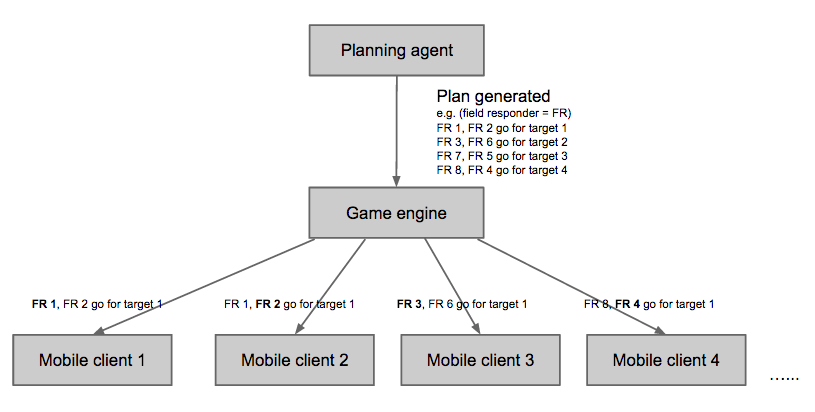
\includegraphics[width=1\textwidth]{img/study2/system/dealingwithplans}
  \caption{Game engine handling plans from agent}
  \label{fig:handlingplans}
\end{figure}

On receiving a instruction from agent, the field responder can choose to either reject or accept the instruction (Figure \ref{fig:study2mobiletask}). In the case of rejection, new plan will be requested and the agent will consider the feedback for the next iteration of task assignment. More importantly, the rejected allocation is used as a constraint within the optimisation run by the planner agent. For example, if two responders (a medic and a soldier) were allocated a task and the solider rejected it, the planning agent would return a new task allocation with the constraint that this soldier should not be allocated this task. The instructions sent to field responders is also displayed in the HQ interface for monitoring purpose. The task allocations are represented as yellow lines connecting players and their targets (Figure \ref{fig:study2mobiletask}). Only one task allocation is displayed at one time, HQ player can click on the `show' task button on player status panel (top right) to chose whose task to be shown.  \\

\begin{figure}[h]
  \centering
  \fbox{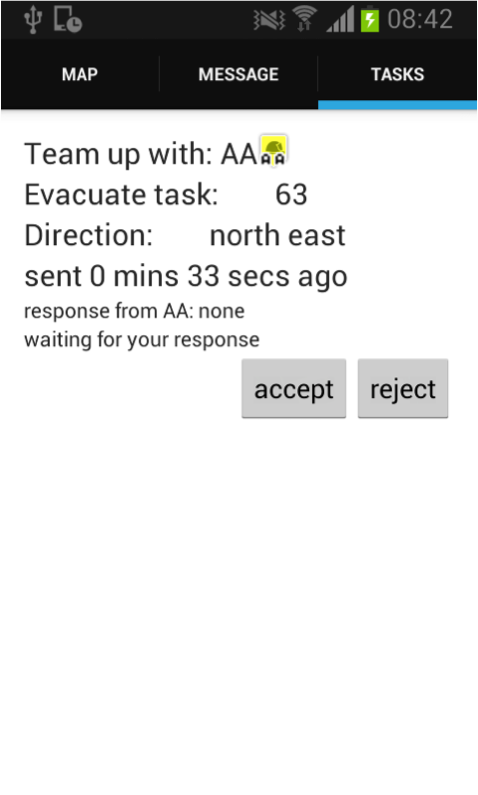
\includegraphics[width=0.4\textwidth]{img/study2/system/mobiletask}}
  \caption{Mobile task interface in study 2}
  \label{fig:study2mobiletask}
\end{figure}

\begin{figure}[h]
  \centering
  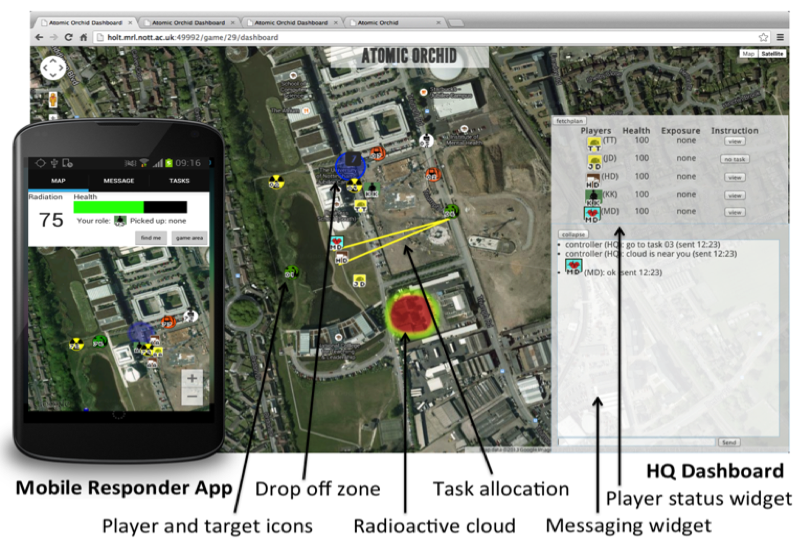
\includegraphics[width=1\textwidth]{img/study2/system/HQ}
  \caption{HQ and mobile interfaces in study 2}
  \label{fig:study2HQ}
\end{figure}


\subsection{Interface improvement}\label{sec:studytwointerface}
Apart from the integration and feedback system, two small modification of the interface is inspired by the requirements of coordination system generated in the previous study (Section \ref{sec:study1requirements}). Firstly, all icons of targets are now marked by a unique target number for HQ and field responders to cross-reference. Secondly, all the messages are labelled by timestamps for players to help identify outdated messages (Figure \ref{fig:study2mobilemsg}).\\

\begin{figure}[h]
  \centering
  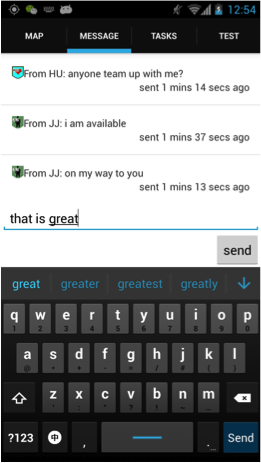
\includegraphics[width=0.4\textwidth]{img/study2/system/mobilemsg}
  \caption{Mobile message interface in study 2}
  \label{fig:study2mobilemsg}
\end{figure}

\section{Study Design}
Study participants were recruited through posters and emails. A total of 18 participants were recruited for 2 sessions of Game play. For each session, there are 1 HQ player and 8 field players. All participants were reimbursed with 15 pounds for 1.5 hours of study. The majority of participants were researchers and students of the local university.  Upon arrival in the HQ (set up in a meeting room at the local university), participants were briefed and asked to consent to participate. Field responders were randomly assigned to all participants (firefighter, medic, transporter, soldier). Roles of field responders were provided with a smartphone; HQ coordinators with a laptop. Game rules and interfaces were introduced, and participants were assisted in setting up their phones and laptop clients. Field responders and HQ coordinators were given 5 minutes to discuss a common game strategy. All field responders were accompanied to the starting point within the designated game area, about 1 minute walk from headquarters.\\

Once field responders were ready to start, HQ sent a ``game start'' message. Gameplay commenced for 25 minutes. A ``Game over'' message by HQ concluded the game. Field responders returned to HQ for the post-game session. A group interview was then conducted after the game play, before participants were debriefed and dismissed.\\

The size of the game area on the local university campus was 400 by 400 meters, without heavy traffic. The terrain of the game area includes grassland, a lake, buildings, roads, and footpaths and lawns. There are two drop off zones and 16 targets. The pilot study showed that this was a challenging, yet not too overwhelming number of targets to collect in a 25 min game session. There were four targets for each of the four target types. The pattern of cloud movement and expansion was the same for both game sessions.\\

%In this study, we aimed to probe a straightforward [interaction design] between a planning support agent and human teams (Fig. 1). The interactional design is designed to facilitate the division of labour between humans and agent: a planning agent routinely assigns tasks to distributed responder teams, while human coordinators (the HQ) monitor and support the task execution by responding to arising contingencies. The agent is designed in a way to take into account simple human feedback, i.e., a field responder can either reject or accept their task assignment. The agent will consider the feedback for the next iteration of task assignment. \\

%By examining the socially organised interaction between team members occasioned by this interactional arrangement, we aimed to explore social implications of human-agent interaction. In turn, these inform the design of agent-based systems. In the following, we describe the study in detail. \\

%A real-time algorithm was developed to support the coordination problem created by the game mechanic. The coordination problem (described in IV, A) is modelled using a Multi-Agent Markov Decision Process (MMDP) that captures the uncertainties of task execution, extending earlier work [15]. The modelling allows responder actions to be delayed or to fail during the rescue process. The MMDP modelling leads to a large search space, even with a small-sized problem. Hence, we devised an approximate solution to save computation time, which can be executed to support real time planning. The planning algorithm takes into account both time (cloud and human movement speed) and spatial (path planning for responders) constraints. The planning algorithm run by the planning agent produces high task allocations that minimise the travelling distance of first responders, and maximise the number of targets rescued. Before the agent was deployed to support human teams in the game setting, computational simulations were used to benchmark our MMDP algorithm against greedy and myopic methods (see Table 1). The results confirm that our algorithm produces efficient task allocations. \\

%In their mission to rescue all the targets from the disaster space, a centrally located HQ and the planning agent support the responders on the ground. In what follows, we present the player interfaces and the interactions with the planning agent. A demo video can be viewed at http://bit.ly/1ebNYty.\\

%First responders are equipped with a mobile responder tool (Fig. 2) providing sensing and awareness capabilities in three tabs (Geiger counter, map, messaging and tasks). The first tab shows a reading of radioactivity, player health level (based on exposure), and a GPS-enabled map of the game area to locate fellow responders, the targets to be rescued and their drop off zones. The second tab provides a broadcast interface to message fellow first responders and the HQ. The third tab shows the team and task allocation dynamically provided by the agent that can be accepted or rejected. Notifications are used to alert both to new messages and task allocations.\\

%HQ controls the HQ dashboard that provides an overview of the game area, including responders real-time locations (Fig. 2). The dashboard provides a broadcast messaging widget, and a player status widget so that the responders exposure and health levels can be monitored. HQ can further monitor the current team and task allocations to individual responders by the planning agent (by using buttons in the player status widget). Crucially, only HQ can see the radioactive cloud, graphically depicted as a heatmap. The rationale was to entice frequent communication between field responders and HQ.  \\

\section{Data analysis and results}
Here, we present findings from interaction analysis that reveal how team coordination was achieved. Overall, responders rescued 12 and 11 targets in session A and B respectively, out of 20 targets in total per session. No player was incapacitated in the two sessions. The planning agent sent a total of 51 instructions (Figure \ref{fig:study2agentInstructions}), 24 of which are accepted and 11 of them are rejected. The remaining 16 instructions does not receive complete response (at least one of the player did not reply). A total of 21 instructions are finished successfully, versus only 2 of the targets are saved without agent. The 19 instructions are unsuccessful, Some of which are ignored or violated by players and some of them are overridden by agent in the replanning process due to change of circumstance.\\

\begin{table}[h]
\footnotesize
\begin{tabular}{llll}
\multicolumn{1}{l|}{} & Saved targets & Incapacitated players & Average Health \\ \hline
\multicolumn{1}{l|}{Session A} & 12 (out of 20) & 0                    & 80/100             \\ 
\multicolumn{1}{l|}{Session B} & 11 (out of 20) & 0                    & 82/100             \\ 
\end{tabular}
\caption{Overview of game results}
\label{tab:gameResults1}
\end{table}

\begin{figure}[ht]
 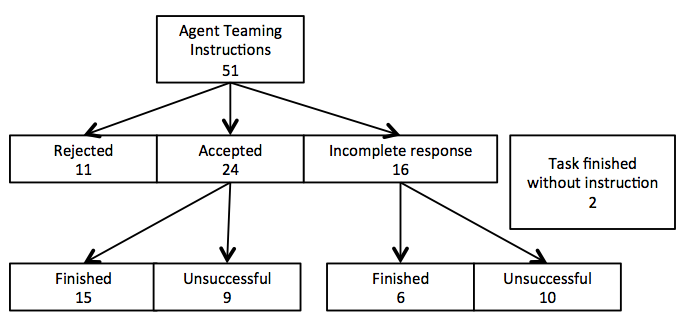
\includegraphics[width=1\textwidth]{img/study2/system/agentInstructions}
\caption{Overview of agent instructions}
\label{fig:study2agentInstructions}
\end{figure}

In what follows, we presents selected episodes of game play to reveal how teams accomplish the tasks in the rescue mission, particularly focusing on the social organisation of interaction with and around the agent instructions. The order in which we present the episodes follows the common practice of moving from exhibits of typical/unproblematic instances, via more complex/difficult instances, to exhibits that display problematic interaction or even complete breakdowns. In the episodes, players can be uniquely identified by their initials. Targets are denoted by their unique numeric target id. Task assignments from the agent are represented as two initials and one target id connected by a rightward arrow. For example, the notation PC, CR -> 22 means player PC and CR are instructed to team up and go for target 22. A standard orthographic notation \cite{Jordan1995} is complemented by timestamps [0:00], and system messages from remote players and HQ.  

\subsection{Assigning task assignments to existing teams}
The following episode depicts a team of two dropping off a target and planning the next step.\\

\noindent\texttt{\textbf{Episode 2.1}\\
\emph{[0:00] The team dropped off a target.}\\
\textbf{PC:} I think we dropped off now. Ok. \\
\emph{ [0:07] The team receives a new agent instruction: PC, CR -> 22}\\
\textbf{PC:} I have a task now (3.0) ((studying screen)), I need to go with CR to 22. Are you CR? (Figure \ref{fig:study2ep11})\\
\textbf{CR:} Yes.\\
\textbf{PC:} go 22.\\
\textbf{CR:} We have done 22.\\
\textbf{PC:} Oh (1.0), no (2.0) 22 is there ((pointing to direction of 22)), Let`s go ((PC leads the way, they start walking to 22))\\
\textbf{PC:} Right this way. (Figure \ref{fig:study2ep12})\\
\emph{ [0:28] The team finishes the task assigned by the agent.}\\
}

\begin{figure}[ht]
\centering
 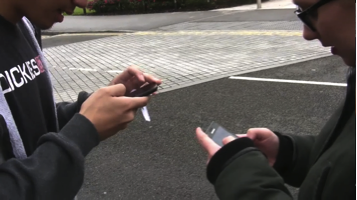
\includegraphics[width=0.7\textwidth]{img/study2/ep1/ep11}
\caption{episode 2.1, CR (Left) and PC (Right) studying screen together after drop off.}
\label{fig:study2ep11}
\end{figure}

\begin{figure}[ht]
\centering
 
\includegraphics[width=0.7\textwidth]{img/study2/ep1/ep12}
\caption{episode 2.1, PC (Right) leading the way to new target.}
\label{fig:study2ep12}
\end{figure}

At the beginning of this episode, the team (PC, CR) drops off a target at a drop off zone. Player PC vocalises that they have finished the task (PC: I think we dropped off now. OK).  After about 7 seconds, PC says she received a new task allocation from the agent (PC: I have a task now). PC confirms the initials of the other player (CR), and suggests CR to join her to go for target 22. The action is consistent with the agent instruction (PC, CR -> 22), suggesting that PC has read through the instruction and decided to follow it. CR said that they have already finished target 22 (CR: We have done 22), which indicates he is confused about the current task allocation. PC resolves the confusion by pointing in the direction of 22 and repeating to go for it. Later, the team successfully drop off target 22 as instructed by the agent.\\

The episode shows how an agent instruction is brought up and followed by a team in relative straightforward manner. The instruction was delivered immediately after the drop off of a previous target (7 seconds after). PC successfully locates the new target in the instruction and leads the team to pick it up. Although CR is confused at first, PC manages to rectify CR mistake and they finish the task successfully. \\

This episode is a typical case of task assignment to existing teams, i.e. the agent sent a new task to a team immediately after they finished their previous task. Out of a total of 51 agent instructions, 23 fall into this category. The rate of compliance is high for these cases of task assignment to existing teams (21 out of 23; 91\%). \\

\subsection{Task assignments involving team reformation}
Unlike episode 2.1, sometimes the agent instruction implies players need to disband and form new teams after finishing their previous task, in order to enact the computationally optimal plan. 10 out of 51 agent instructions fall into this category (Table \ref{tab:compliancerate}). The compliance rate of instructions that require reteaming (50 percent) is substantially lower than compliance of instructions where players can stay in the same teams (91 percent). The following episode depicts a typical case in which team reformation fails.\\

\begin{figure}[ht]
 
\includegraphics[width=1\textwidth]{img/study2/ep2/ep21}
\caption{episode 2.2, players from left to right: LT, SS, CR, PC. LT  walking around the team, her body orientation suggesting attempts to leave the group.}
\label{fig:study2ep21}
\end{figure}

\noindent\texttt{\textbf{Episode 2.2}\\
\emph{[0:00] After a target drop off, LT and SS joined PC and CR at drop off zone.} \\
\emph{ [0:24] HQ sent message A: LT, if you think you have the stamina to run to 10 around the north of the lake do so now with a firefighter. }\\
\emph{ [0:28] Agent instruction received:  NK, LT -> 16 }\\
\textbf{LT:} They said ((reads out aloud HQ message A)) \\
\emph{[0:35] CR ((facing LT)): Shall we go get 10}\\
\textbf{LT:} Mine is 16. \\
\emph{[0:38] HQ sent message B: Avoid 17 at all costs (...) I`d avoid 10, too.}\\
\textbf{CR:} ((read out HQ message B)) avoid 10 now. \\
\emph{[0:55] New agent instruction received: NW, LT -> 15}\\
\textbf{LT:} 15!\\
\emph{[Fig. 3] LT keeps walking and turning back and forth from others. PC and SS discuss next steps, LT does not engage in the discussion with them. }\\
\emph{[1:12] SS ((facing PC)): Shall we go get 19? ((turning towards LC and CR)) are you going to 10 or something? }\\
\textbf{CR:} Eh::, HQ said no. [referring to message B]\\
\emph{[1:24] SS and PC decide to go for target 19, and leave.}\\
\emph{[1:29] NW sent message: LT where you}\\
\textbf{CR:} ((facing LC)) Are you LT? \\
\textbf{LT:} Yes. \\
\textbf{CR:} NW is looking for you. \\ 
\textbf{LT:} Yah thanks. ((turning away from CR)) Ah::. I will go towards them.  ((starts walking)) \\
\textbf{CR:} Okay. Do you want company?\\
\textbf{LT:} ((turning back towards CR)) Yeah. \\
\emph{CR and LT leave drop off zone together to find NW.}\\
}

The episode begins with a recommendation by HQ to LT to go for 10 (message A). The message is topicalised by LT, but it is soon overridden by an agent instruction (NK, LT -> 16). When CR proposes to team up with LT to go for target 10, LT declined (LT: mine is 16). HQ then withdraws its previous suggestion to go for 10 in message B. Shortly after; a new instruction (NW, LT-> 15) prompts LT to read out the target number (15), but she fails to raise the other players attention. While other group members engaged in planning next steps, LT does not engage and keeps looking around. She can be seen turning and walking back and forth (Figure \ref{fig:study2ep21}). Perhaps LT is trying to locate the player NW who she had been instructed to team up with. LT does not take any action until prompted by CR (CR: are you LT? NW is looking for you). Then, LT begins to walk to find her teammate. However, when she finally manages to meet up with NW two minutes later, NW has already been assigned another task. \\

On one hand, LT seems to feel obliged to follow the agent instructions. She turns down other teaming invitations and appears to try to look for NW in her immediate vicinity, indicating difficulty with locating teammates out of sight (despite the real-time location map). On the other hand, her body orientation displays a sense of attachment to the existing group. Her indecisive walking and turning back and forth suggests she struggles to leave. She does not leave the group to follow the instructions until prompted by someone. When CR points out NW message, LT does not answer the message either. The episode illustrates a combination of interactional troubles as a result of which the reteaming fails: being attached to the local group, struggling to locate teammates out of sight, and failing to reciprocate messages. \\

Further, we found the distance between instructed players to be a key factor in successful reteaming. That is to say, if instructed players are not within line of sight, the rate of non-compliance with the agent instruction is high. Take episode 2.2 as an example, player LT was instructed to team up with a distant player twice. Neither one of the instructions was successfully implemented. Overall, there were 17 agent instructions that implied teaming with distant players; only 1 of them were actually followed by players. Players explicitly rejected 11 of them by pressing the rejection button; the other 5 were not followed without an interface action (nether accept nor reject).\\

\subsection{Task assignments involving task interruption}
In some other cases, the agent also sent new instructions to teams that had already commenced their task; that is, teams were interrupted by the new instructions. The following two episodes C and D describe how players handled task interruptions caused by the agent.\\

\begin{figure}[ht]
\centering

\includegraphics[width=0.5\textwidth]{img/study2/ep3/ep31}
\caption{episode 2.3, AW (right) leads the way, heading to target 44 as instructed.}
\label{fig:study2ep31}
\end{figure}

\begin{figure}[ht]
\centering

\includegraphics[width=0.5\textwidth]{img/study2/ep3/ep32}
\caption{episode 2.3, After the team received an instruction to disband, AW (right) and HB (left) simultanously turn back and start walking back to the drop off zone, displaying bodily alignment.}
\label{fig:study2ep32}

\end{figure}

\noindent\texttt{\textbf{Episode 2.3}\\
\emph{ [00:00] HB, AW at drop-off zone, new instruction received: AW, HB->44} \\
\textbf{HB:} Alright, who is AW? \\
\textbf{AW:} Me.\\
\textbf{HB:} let's go southeast (the direction of target 44).\\
\emph{[00:07] AW, HB looking at their screens.}\\
\textbf{[00:26] HB:} There is no 44.\\
\textbf{AW:} down there.\\
\textbf{HB:} Ok, yea, yea, yea (0.5), I can`t see, Oh, there, yea, let`s go.\\
\emph{[00:35] [Fig.4] Team begins moving towards 44.}\\
\emph{[00:48] HQ sent message: Target 42 and 44 is not reachable.} \\
\textbf{AW:} ((reads out the message))\\
\emph{AW and HB stopped walking.}\\
\emph{[00:52] New instructions received: AW, KD -> 44, HB, AR->31}\\
\textbf{AW:} I got a new instruction.\\
\emph{[Figure \ref{fig:study2ep31}] AW and HB simultaneously turn and start walking back towards the drop off zone.}\\
\textbf{HB:} I need to team up with AR.\\
\textbf{AW:} I need to team up with KD! Oh, it is 44 again.\\
\emph{ [01:01] AW, HB arrived at drop off zone, met AR, KD.} \\
\textbf{HB:} AR?\\
\textbf{KD:} AW? We have got (1.0), 44, right?\\
\textbf{AW:} It said 44 is not reachable, but I got it again, so, let`s try.\\
\textbf{KD:} Alright. \\
\emph{[01:14] AW, KD begin walking to 44, AR, HB team up as well.}\\
}



This episode begins with an instruction (AW, HB -> 44) from the agent. At that moment, there were 5 players at the drop off zone (AR, KD, LC, HB, AW). Immediately after the instruction, HB starts looking for AW in the local group. Shortly after, AR and HB team up to go for 44 as instructed.  However, 13 seconds later the team is interrupted with a HQ message telling them not to go for 44 (Target 42 and 44 is not reachable). Four seconds later, a conflicting agent instruction was delivered, implying they disband the team (AW, KD -> 44, HB, AR->31) but still pursue the target 44. At first, AW stops walking and topicalises the instruction (AW: I got a new instruction), followed by both teammates simultaneously turning towards each other (Figure \ref{fig:study2ep31}, \ref{fig:study2ep32}). The bodily alignment in the action suggests agreement to follow the new instruction. On their way back to drop off zone, HB and AW confirm their intentions (HB: I need to team up with AR, AW: I need to team up with KD!). In this case, the teammates respond to the interruption by mutually agreeing to abandon the current team and task in favour of following the new assignment. \\

It should be noted that the interruption was received only 17 seconds after the team commenced the task, probably contributing to a low perceived cost of abandoning the current task. Further, all players involved in the subsequent reteaming were not far away from each other. AW and HB had not walked too far from the drop off zone; so everyone was still within line of sight, further facilitating successful reformation. \\

\subsection{Disagreement on task interruption}

\noindent\texttt{\textbf{Episode 2.4}\\
\emph{[Following on from Episode 2.3]}\\
\emph{AW, KD on their way to target 44.}\\
\emph{[01:39] New instruction received again, AW, HB -> 44, AR, KD ->31}\\
\textbf{AW:} new instruction, HB and 44 again, haha.\\
\emph{AW turns back towards drop off zone immediately.}\\
\textbf{KD:} AR and 31 ((Reading his new instruction)) ehh, have they gone? Because we can just decline and carry on.\\
\textbf{AW:} Ok, I rejected it. \\
\emph{AW turns back towards KD, who also rejects the new instruction. They resume their walk to 44.}\\
\emph{[01:54] New instruction delivered to AW (AW, YF ->46)}\\
\textbf{AW:} new instruction 46, yeah! ((team stop walking))\\
\textbf{KD:} Do they know we are already on the task?\\
\emph{[02:00] New instruction delivered to AW (AW, LC ->37)}\\
\textbf{AW:} yea, but I think, Oh, no, got new instruction again, (team up with) LC.\\
\emph{[02:13] AW starts walking to LC, who is at drop off zone within line of sight, leaving behind KD.}\\
\textbf{KD:} ((reads out HQ message)) AW and KD you won`t reach 44.  Alright, Let`s go to 46.\\
\emph{AW ((turning back towards KD)): I don`t know, I got a new task with LC.}\\
\textbf{KD:} Ahh, I do not have a task. \\
\emph{AW turns and walks towards LC again. KD follows.}\\
}


In this fragment, we can observe disagreement and negotiation of team reformation. Following episode 2.3, player AW disbands his team with HB and teams up with KD. However, 20 seconds after the reformation, AW is instructed to abandon the on-going task again. AW laughs, but turns back to find player HB again. Before AW sets off, KD disagrees with the new instruction and proposes to reject it (Ehh, have they gone? Because we can just decline and carry on). AW accepts KDs suggestion and turns back to KD.\\

After the rejection, AW receives 2 consecutive reteaming instructions from the agent, finally teaming them up with LC, while KD does not receive another instruction. KDs question (Do they know we are already on the task?) suggests that he might think the agent is unaware of their situation, and that he disagrees with disbanding the existing team. In spite of KDs disagreement, AW declares his intention to follow the new instruction (got new instruction again, [team up with] LC) and he turns to find LC. However, KD ignores this (KD: Alright, Lets go to 46), indicating he does not agree with AWs intention to disband the team. AW interjects (I dont know, I got a new task with LC), and continues to walk towards LC, denying KD. As KD realizes he is without assignment (Ah, I do not have a task), he follows AW to find LC. \\

In this episode, teammates agree to reject the first task assignments. We found task interruption could be a major reason to reject new instructions. 10 out of 11 rejected instructions are associated with task interruption. In an extreme case (not pictured), one team reached an agreement to ignore any agent instructions after the agent tried to interrupt the teams on-going task. \\

In the end, the player that received the new instruction disagrees with his teammates suggestion to ignore the instruction and decides to leave the current team. The team is disbanded in disagreement, in contrast to episode 2.3 where both teammates agree to leave the team after both received new instructions at the same time. Here, the teammates spend a fair amount of time arguing whether to follow or ignore instructions, hinting at the hidden social cost of agent coordination algorithms when applied to human teams. \\

Overall, the majority of new instructions that interrupted on-going tasks required team reformation. When tasks were interrupted, the rate of compliance (22 percent) is substantially lower than when teams were required to reform after a task was completed (50 percent). Task interruptions were also much more likely to lead to rejection of the new assignment. 10 out of 11 assignments that interrupted tasks were rejected.\\

\subsection{The headquarters}

HQ sent a total of 147 messages in the two sessions. We identified 50 assertives and 68 directives in two sessions through speech act analysis. The majority of assertives were focused on providing situational awareness and safe routing the responders to avoid exposing them to radiation. E.g. ``NK and JL approach drop off 6 by navigating via 10 and 09.'' Or ``Radiation cloud is at the east of the National College.''\\

16 out of 68 directives were directly related to task allocations and teaming, which is substantially less then the number of agent instructions (51). Among the 16 directives, HQ sent 11 direct instructions to the field players (e.g. SS and LT retrieve 09), while the remaining 5 are related to forward planning, (e.g., DP and SS, as soon as you can head to 20 before the radiation cloud gets there first). 6 of the HQ instructions are consistent with agent instruction, while 5 other HQ instructions override the agent instructions. It is worth mentioning that field players implemented only 5 out of 16 HQ instructions. In the interview, HQ reported that they felt they supported the agent rather than take control. \\

Insert a diagram here.



\section{Discussion}
In the previous sections, we described how the agent guidance is interleaved with the social interaction, in which teammates organise the task planning and execution. We found that while the agent supported division of labour, the agent guidance had various social implications. We now reflect on (A) how division of labour is achieved; (B) the social implications and hidden cost incurred by team reformation and task interruption; and (C) the limited feedback mechanism. \\

\subsection{Division of labour between the agent and the human teams}
Overall, players followed 30 out of 51 agent instructions, out of which 21 tasks were completed according to the instruction (success rate of 70 percent). Only 2 targets were evacuated without agent instruction (Figure \ref{fig:study2agentInstructions}), which indicates that, to a large extent, the agent successfully supported routine task planning activities. Episode 2.1 demonstrates a typical case of division of labour: the agent handles planning of teaming and task assignment, freeing the team to focus on other issues such as navigation (identifying the target on the interactive map and finding directions) and organising team meet up.  The following of agent instructions speaks of players trust in the agents decisions. In the 30 cases where instructions were followed, we can observe similar patterns of labour division.\\

The distribution of HQ messages may also indicate a division of labour between HQ and the agent. Only a small proportion (16 out of 147) is directly related to task assignment, indicating routine task allocations were delegated to the agent. A relatively large proportion (118 out of 147) of messages are used to provide situational awareness and safety routing the responders to avoid radiation exposure. However, the fact that only 5 (out of 16) HQ instructions are implemented suggests that HQ was unable to effectively override the agent when they wanted to. This fact highlights that the planning agent plays a strong role in the control loop, compared to the human coordinators in the HQ. The planning agent can directly instruct field responders without consent of the HQ, and the HQ does not have an effective way of overriding the agents decision. \\

\subsection{Hidden costs of team reformation and task interruption}\label{sec:study2social}
With this division of labour introduced in Section \ref{d}, it appears that system can successfully generate plans for human to ``executes''. However, Following the view of situated actions \cite{Suchman1987}, The plan is actually a resource in the situation that human can leverage or not. In what follows, we reveal the significance of the plan in determining human's actions varies based on the social situations the players are in. 

First, while team compliance rate with agent instructions was high when no reteaming was required (91 percent), we found that the rate of compliance with agent instructions is much lower when team reformation is involved (50 percent), and even lower when in addition an on-going task is interrupted (22 percent) (Table \ref{tab:compliancerate}). Our interaction analysis shows the ways in which team reformation and task interruption are associated with hidden costs in the social organisation of team performance.  \\

\begin{table}[h]
\footnotesize
\begin{tabular}{l|ccc}
Context                   & \multicolumn{1}{l}{Instructions} & \multicolumn{1}{l}{Followed by FR} & \multicolumn{1}{l}{Compliance rate} \\ \hline
Instructing existing team & 23                               & 21                                 & 91\%                                \\
Require team reformation  & 10                               & 5                                  & 50\%                                \\
Interrupting tasks        & 18                               & 4                                  & 22\%                                \\
Total                     & 51                               & 30                                 & 59\%                               
\end{tabular}
\caption{Compliance with agent instructions by context}
\label{tab:compliancerate}
\end{table}

We found that team disbanding can be difficult. Players have to make their actions accountable to gracefully disengage from an existing team to avoid breaching social norms (e.g., politeness). Members have displayed a sense of attachment to a local group (episode 2.2), which delayed the task substantially until the team reformation failed. Despite interrupting an on-going task, new instructions for both teammates can facilitate smooth, mutually agreed disbanding (Episode 2.3), while instructions for only one member have coincided with interactional trouble, disagreement and delays (episode 2.4). \\

The impact of attachment between co-located teammates was further amplified by distance between proposed teammates. While they frequently accounted for actions with co-located players, they did not make their actions equally accountable to remote team members. For example in episode 2.4, the agent interrupted the local teams task and instructed them to team up with distant players. The co-located team decided to reject the instruction without contacting the potential teammates they rejected. The system lacked support of accountability between remote members. \\

A further observation is that players were unwilling to give up on-going tasks after a certain time. In episode 2.4, the teammates first agree to ignore new instructions. This preference to stick with on-going tasks may also explain the high rejection rate for instructions involving task interruptions. \\

The social organisation of coordination reveals implications for the simplistic model of interaction held by the agent. The agents algorithm re-plans and reshuffles teams, in order to optimise group performance by minimising the travel distance to the targets. However, our study has revealed the ways in which social norms and the accountability of social conduct get in the way. This raises questions of the effectiveness of approaches that treat coalition formation of humans as unproblematic. The agent does not consider the social cost of team reformation and task interruption. Our field study has shown that the social process to disengage from groups and on-going tasks can be costly. The tension between the social process and the model held by the agent echoes the notion of workflow from within and without \cite{Bowers1994}. The authors point out that models imposed by technology (from without) may come into tension with the actual workflow achieved through methods internal to the work (from within). 



\subsection{Feedback to the agent}\label{sec:studytwofeedback}

To recap, a feedback mechanism is included in the interaction design to give responders some control over the task assignment (Section \ref{sec:study2feedback}). On receiving an instruction, players can either accept or reject instructions. On rejection of a task allocation, a new plan is requested. The rejected allocation is, in turn, used as a constraint within the optimisation run by the planner agent, which means the rejected target will not be assigned to the rejecting player for a while (1 minute). \\

Our observations show there may be a significant cost associated with rejection. Overall, 6 out of 25 re-plans were triggered by rejections. In turn, tasks were re-assigned to all players. Frequent new instructions may cause extra coordination overhead (time spent on interpreting new instructions, more team reformation and task interruptions, and over-constrain the planning). Players did not seem to be aware of the implications that their rejections had on others.\\
 
We also found that players expectations of the rejection were not always aligned with its actual effect. Instructions involving reformation and interruption are more likely to be rejected. Players statements indicate they perceive the rejection as a way to reverse to previous states (see episode 2.4). Other statements indicate rejections were expected to pair them with a new teammate instead of a new target. The mismatch between expected and actual effect highlights the lack of intelligibility in the current interaction design. We aimed at simplicity (by providing only accept/reject options), which might be important for interaction in time-critical task settings, but it comes at the cost of intelligibility. Therefore, we argue that intelligibility and simplicity need to be carefully balanced according to details of the setting.\\


\section{Design implications}

Our observations reveal the tension between agent planning support and the social organisation of teamwork. The tension does not simply mean the model held by the agent is incorrect; it highlights potential trade-offs we need to consider in system design \cite{Bowers1994,Sukthankar}. Providing a detailed design solution is beyond the scope of this chapter. Instead, we propose three design implications to scaffold the division of labour when building agent-based planning support for human teams.\\

\subsection{Achieve common ground}  
Two main issues arose that challenged this basis for collaboration \cite{Bradshaw2011}. Firstly, a notion of the social cost associated with instructing teams should be taken into account when designing planning agents. For example, disbanding teams can be difficult and time-consuming as it is governed by rules of social conduct and etiquette, particularly where the new teammates are out of sight or only one of the teammates received a new instruction. Secondly, a mismatch between the expected and actual function of rejections further shows intelligibility needs to be improved. Therefore, we suggest the design of agent support that a) takes social factors into consideration (e.g., ensuring team disbanding is facilitated by reteaming both teammates at the same time; avoiding task interruptions etc.), and that b) agent functionality is appropriately surfaced to help achieve common ground (e.g., by providing explanations of agent action at the interface level).

\subsection{Facilitate accountability}
while the rules of social conduct ensured accountability of action among co-located teammates, we found the impact of rejections on remote players was not properly appreciated; nor did the interaction design support making these rejections accountable. Therefore, we believe the interaction design shall reveal the hidden cost of certain actions (e.g., rejections) to facilitate local decision making accountable to remote team members, ensuring consequences of local decisions for the welfare of all teams are understood. 

\subsection{Balance responsibilities between humans and agent}\label{sec:balanceResponsibility}
 The social implications and other situational contingencies are likely difficult to be modelled computationally. Alternative approaches argue for mixed-initiative  control and flexible autonomy between humans and agents \cite{Bradshaw2011}. The ways in which the HQ used messsages to provide situational information that complemented the agent instructions show that humans are readily able to deal with arising situational contingencies. The division of labour between humans and the agent appeared most effective in that the agent took on routine and repetitive jobs (task assignment), which freed the responders to focus on the situated rescue mission. In our interaction design, the role of the human HQ was relatively weak. For example, the HQ struggled to overwrite the agents instructions through the messaging channel. In the future, we seek to allow the HQ to play a stronger role in the control loop to enable more direct mediation and amendment of agent instructions (e.g., by directly modifying the task assignments, or by adding information relating to the assignments, such as safe routing).
 
%==== what is possible situational contingencies? social implications, coordination overhead incured is hard to be modelled, and other unexpected situational contingencies are hard to be considered by the agent. The example being some players is reluctant to disband team and unwilling to team up with remote players. As they are hard to be considered and model by the agent, HQ's input can be useful to judge the situation and contribute to the planning. In this field trial, The division of labour between humans and the agent appeared most effective in that the agent took on routine and repetitive jobs (task assignment), which freed the responders to focus on the situated rescue mission. However, the HQ is weak in terms of influencing the planning and plan executions. The reason has been summaried in section xxx. Here, we propose some requirements based on the.  ====%

\section{Summary}

In this chapter, we examined how the guidance from a planning agent is handled socially in the Human On-the-loop setting. To support our field trial we integrated a planner agent with AtomicOrchid and modified both mobile and HQ interface to facilitate the On-the-loop interaction pattern between human and agent. Findings from interaction analysis of field observations, triangulated with log files, reveal how the On-the-loop interactions played out. The results of analysis show a division of labour in which the agent takes over the majority of planning activities while field responders only focus on other issues such as finding routes and targets. However, field observations also reveal significant costs associated with instructions that require members to reform new teams, and that interrupt on-going tasks. In addition, some confusions and misunderstanding are also discovered in the human agent feedback loop.Based on the findings, we presented three design implications to consider when creating agent-based planning support systems for human teams, including establishing `Common Ground', facilitating accountability and balancing responsibilities between human and agent.\\


%************************************************
\chapter{AtomicOrchid Study 3: Agent-supported In-the-loop design}\label{ch:studythree} 
%************************************************
This chapter presents the third iteration of AtomicOrchid(AO) field trials. The purpose of these trials is to investigate socio-technical issues relating to agent planning support with a Human In-the-loop interaction design. Based on the On-the-loop version of AtomicOrchid (Section \ref{sec:studytwosystem}), the system have gone through another development iteration to facilitate a In-the-loop interaction pattern. Through interaction analysis of video recordings and game log data, we reveal how this In-the-loop design unfolds and, through a number of critical incidents, how it breaks down. We find that the human coordinator and automated planner agent can successfully work together in most cases, with human coordinators inspecting and `correcting' the agent-proposed plans. However, occasional failures of planning are also observed due to: complacency; silent, missing or invisible information; and limited support for human planning. A workshop with a professional disaster response team is conducted to reflect on realism of AtomicOrchid scenario and raises the challenge to extend this work to more complex but slower paced situations.   \\


\section{Introduction}
Most disaster operations require responder teams to plan and carry out task under spatial and time constraints. which means the teams often have limited resource and personnel to deal with large amount of geopolitically distributed tasks in limited amount of time. How do they optimise the use their rescue resources become computationally complicated problem. Multi-agent system researchers have developed a number of multi-agent task allocation algorithms. As software components, they have all done very well in the computational simulation, therefore there is potential to apply those algorithms to support planning activity of human responder teams. \\

However, these algorithms necessarily depend on abstracted models of the environment and human behaviour which might lead to task allocations that are flawed in practice, due to the contingent nature of situated action \cite{Suchman1987}. We might conjecture that a human coordinator working together with the planning agent could notice and help to deal with such emergent problems. One way in which this working together might be achieved is by placing a human coordinator In-the-loop between the planning algorithm and the physical world. The In-the-loop design pattern assumes the constant HQ supervision and intervention is required to ensure the agent works properly (section \ref{sec:approachPatterns}). In this study, the AtomicOrchid system has evolved from the 2ed game probe in the study 2 (chapter \ref{ch:studytwo}), to facilitate the In-the-loop interaction. The In-the-loop design enables HQ human to involve in the planning process by: \\


%However, there is concern that the algorithms hold over-simplified model of the environment and human behaviours. Therefore, effective interactions with the responder teams may be required to ensure the planning agent actually support (rather than hinder) the planning process of responder teams, which highlights the importance of appropriate interaction design. 

\begin{enumerate}
	\item allowing HQ to review, edit and approve every instructions generated by agent. (Figure \ref{fig:study2InTheLoop} (1)). In extreme cases, HQ can override all agent instructions, i.e. manually allocate all tasks.
	\item allowing HQ to decide when to initiate re-plans. (Figure \ref{fig:study2InTheLoop} (2))
	\item allowing HQ to review feedbacks from field players and how to act on them. (Figure \ref{fig:study2InTheLoop} (3))
\end{enumerate}

\begin{figure}[h]
  \centering
  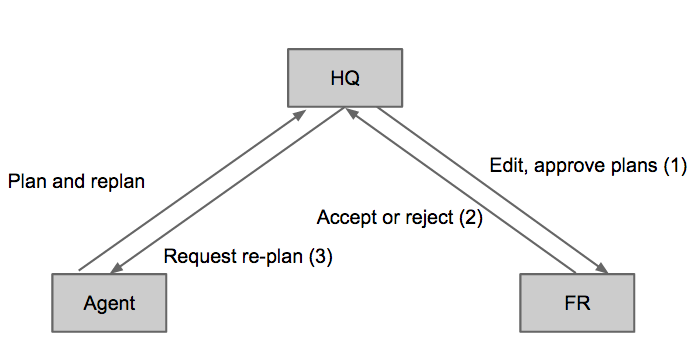
\includegraphics[width=1\textwidth]{img/study3/InTheLoop}
  \caption{In-the-loop interaction design}
  \label{fig:study2InTheLoop}
\end{figure}

Compared to the Human On-the-loop design in the previous study (Section \ref{sec:approachPatterns}) , the major change is the rebalance of responsibilities in the control room (between HQ and agent). The interaction between field responder and the control room is mostly unchanged. Therefore, this study has strong focus on control room interaction compared to the study 2. More specifically, objective of this study is to unpack the human agent interaction in the human In-the-loop paradigm, particularly in the control room, revealing labour division, interactional issues and design implications that can be drawn from the interactions.\\

Findings from the study highlight the processes in which the agent and HQ players collectively generate task assignments for field players. The human coordinator and automated planner agent managed to successfully work together in most cases, with human coordinators inspecting and `correcting' the agent-proposed plans. However, occasional failures of planning are also observed due to: complacency; silent, missing or invisible information; and limited support for human planning. A workshop with a professional disaster response team is conducted to reflect on realism of AtomicOrchid scenario and raises the challenge to extend this work to more complex but slower paced situations. \\


\section{System Evolution}\label{sec:study3system}
The In-the-loop version of AtomicOrchid is not designed from scratch, but evolved from the On-the-loop version introduced in previous study (Section \ref{sec:studytwosystem}). In the study 2, we have observed HQ struggling to get involved in the planning loop even when they want to intervene. Combining the observations from the study 2 and the definition of In-the-loop interaction pattern (\ref{sec:approachPatterns}), we further generate several system requirements for realizing the In-the-loop interaction. \\

\begin{enumerate}
\item HQ should be able to review, edit and approve every instructions generated by agent.
\item HQ should be able to decide when the agent should re-plan. 
\item HQ should be able plan for part of the team, leaving the agent to plan for the team left. 
\item HQ should be able to deliver their assignments(or task cancellation) to FR with a structured presentation. 
\end{enumerate}

The purpose of requirement 1-2 is to give HQ more control over the planning loop, by delegating them the responsibility of final decision in planning. The requirement 3 enables HQ to modify in the agent planning without having to take full manual control of plan generation. The requirement 4 is derived from the observations (study 1 and 2) that HQ struggled to override agent planning through a unstructured text messages. Therefore, we suggest to enable HQ to deliver and cancel their assignments in a structured in the same way that the agent do. Two interfaces are designed for the 2 HQ players in the control room. The task assignment interface provides a set of interface functionalities supporting task allocation activities, while the situational awareness interface provides game status and a broadcasting message channels.  \\

% the mobile responder app
\begin{figure}[h]
  \centering
  \includegraphics[width=1\textwidth]{img/study3/system/interfaces}
  \caption{The mobile responder app}
  \label{fig:mobileResponderApp}
\end{figure}

%1. Plan request:  HQ can request planner to generate plan (at 1). Agent conducts task optimization based on current task status, and proposed on optimal plan to HQ for review.\\
%2. Plan review: HQ can choose make some minor edits to agent proposed plan. Alternatively, the HQ can propose some assignments, and re-initiate step (1) to let the agent conduct partial planning for the rest of the team (explain for partial planning, see section x). \\
%3. Plan approval: If HQ is satisfied with the plan, he/she can send the plan to field responders for execution. \\
%4. Feedback and further communication: When Field responders receive plans, they can communicate with HQ to provide feedbacks and request clarifications. Based on the task execution status and feedbacks, HQ can decide to initiate to step (1) again for re-planning. \\


\subsection{Interfaces}
This section describes three game interfaces used by players, which includes mobile responder interface for field responders, task assignment interface and situational awareness interface for HQ players.\\

Compared to the On-the-loop version of AtomicOrchid, the mobile interface is mostly unchanged except for the HQ task tab (see figure \ref{fig:study3mobileInterface}). The task tab now displays a task with text description and map visualisation of task on the top. The bottom half of the interface is a message box showing task-specific information from HQ. It should be note that the HQ can still send broadcast information (visible to everyone), which will be displayed in the chat tab. \\

\begin{figure}[h]
  \centering
  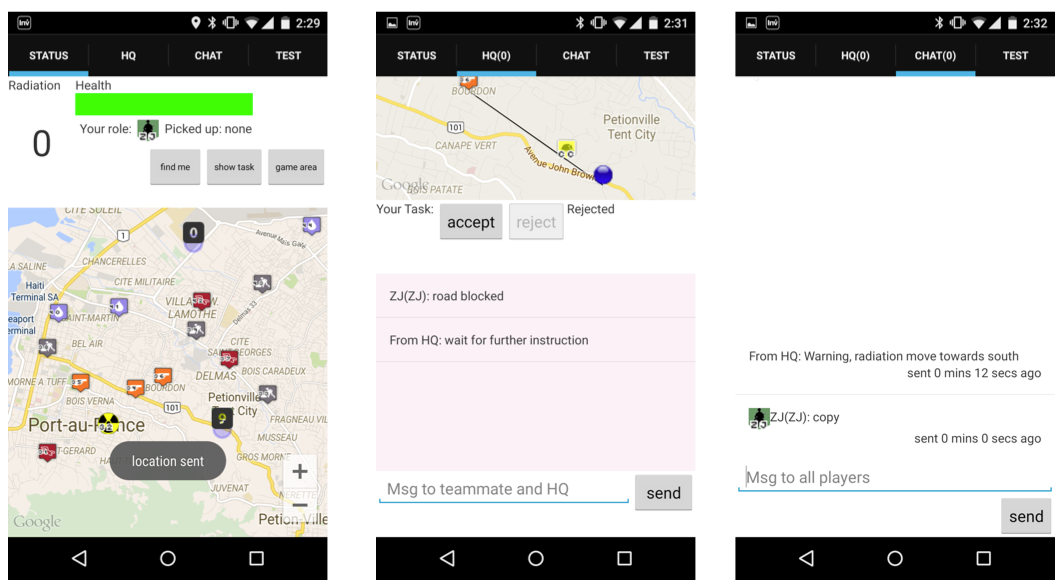
\includegraphics[width=1\textwidth]{img/study3/system/mobileInterface}
  \caption{Mobile interface in study 2}
  \label{fig:study3mobileInterface}
\end{figure}

The situational awareness interface is the same as the HQ interface used in study 2 (Study \ref{sec:studytwointerface}). It provides information for game status monitoring, and a broadcast message channel for communicating with field players.\\

\begin{figure}[h]
  \centering
  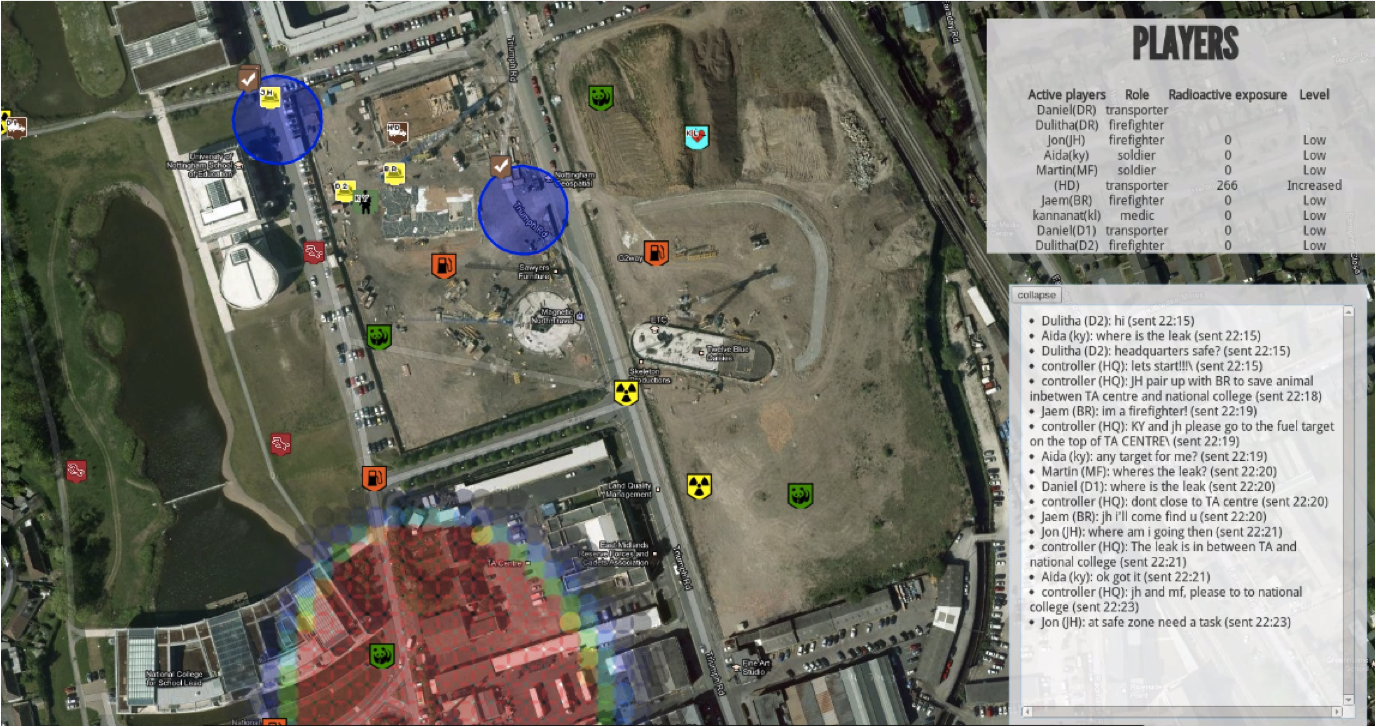
\includegraphics[width=1\textwidth]{img/study3/system/HQ2Interface}
  \caption{Situational awareness interface operated by HQ2}
  \label{fig:study3SAinterface}
\end{figure}

The task assignment interface is created to support In-the-loop interaction with Agent. As an overview, the interface has a map on the left (Figure \ref{fig:study3TAinterface}). Player/target locations, assignments are presented on the map. At right side of the interface is a task assignment panel. The left (1) column of the panel shows pending assignments while right column (2) shows existing task status. Figure  \ref{fig:study3TAinterface} (5) shows an example of a proposed task assignment: player MD and GO are assigned to target 07. Within each confirmed task assignment (6) a feedback indicator indicates the field player`s response to this assignments (no response, reject, accept).\\

\begin{figure}[h]
  \centering
  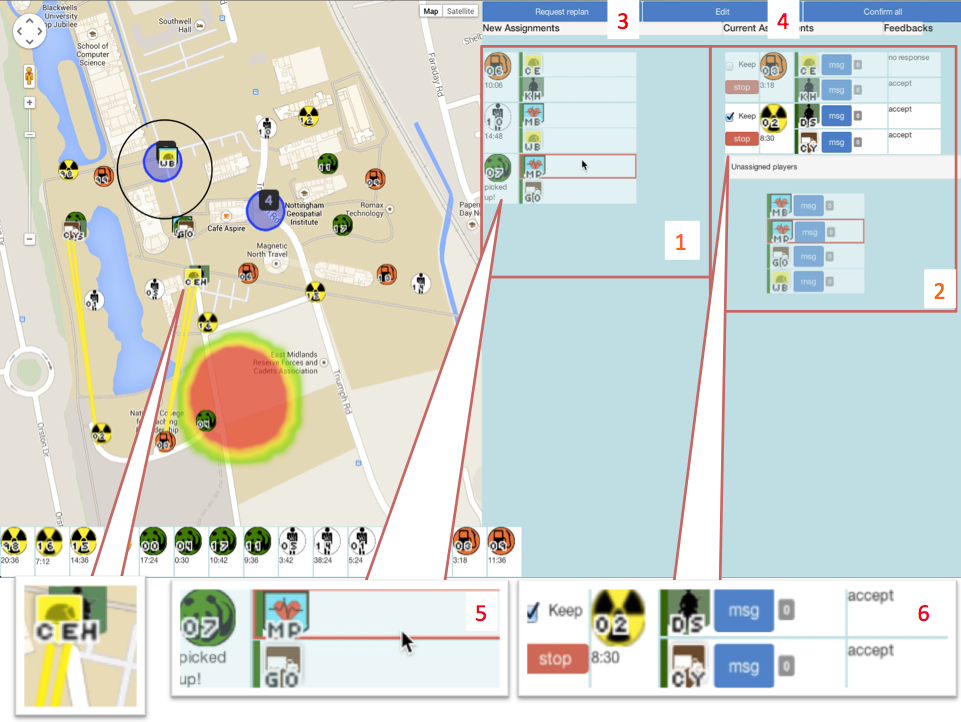
\includegraphics[width=1\textwidth]{img/study3/system/HQ1Interface}
  \caption{Interfaces in study 3}
  \label{fig:study3TAinterface}
\end{figure}

\begin{figure}[h]
  \centering
  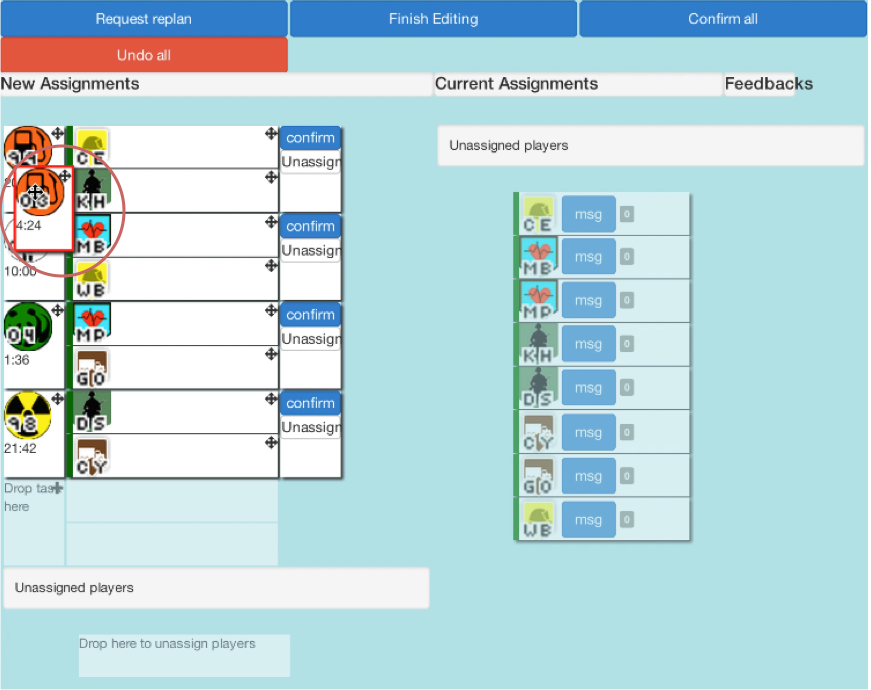
\includegraphics[width=0.5\textwidth]{img/study3/system/editmode}
  \caption{Edit mode of task allocation interface}
  \label{fig:study3editmode}
\end{figure}

\begin{figure}[h]
  \centering
  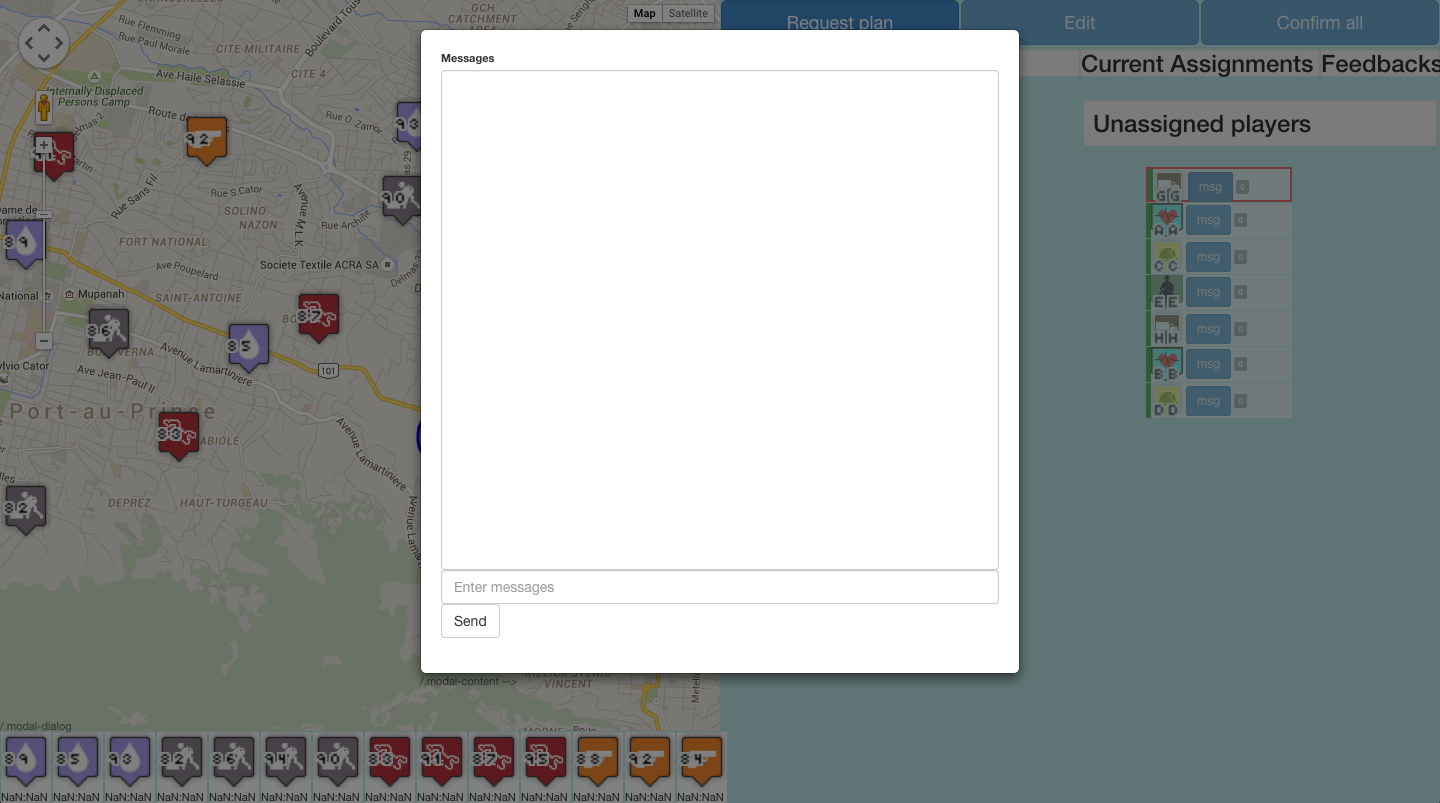
\includegraphics[width=1\textwidth]{img/study3/system/msgmode}
  \caption{Pop up messaging panel}
  \label{fig:study3msgmode}
\end{figure}


\begin{enumerate}
\item Plan request button: \\
This button triggers agent re-planning. The agent will calculate an optimized plan based on task status, and present it to the HQ on the pending panel. The button allow HQ decide when to initiate a re-plan. (Figure \ref{fig:study3TAinterface} (3))\\

\item Plan keeping checkbox:\\
These checkboxes are attached to every task assignments in the confirmed panel. If the checkbox is ticked, the planner will keep the corresponding assignment in next re-planning. In other words, the planner will keep the assignment fixed, performing partial planning for the rest of the team. (Figure \ref{fig:study3TAinterface} (6))

\item Plan edit panel: \\
Manual plan edits will be activated by clicking the `edit' button (Figure \ref{fig:study3TAinterface} (4)). The assignments in pending area will change to edit mode. Assignment can be created, modified and deleted through drag and drop interaction. (Figure \ref{fig:study3msgmode}) \\

\item Plan approval button: \\
This button approves all pending assignments. All pending assignment will switch to confirmed area. Alternatively, assignments can be approved individually by clicking individual confirm button on the pending assignment when the edit mode is activated. \\

\item Text messaging panel:\\
The messaging panel can be toggled by clicking msg button on the confirmed assignments (Figure \ref{fig:study3TAinterface} (4)). The panel is supposed to be used for assignment-specific information. Therefore, the messages in this plan are only visible to the two involved players and HQ. (Figure \ref{fig:study3msgmode}) \\

\item The Feedback indicator:\\
The feedback indicators are attached to the right hand side of the confirmed assignments. The field players can easily provide feedbacks of their assignment through mobile responder interface (introduced later). There are three possible values for the indicator (no response, reject, accept). Because rejections typically indicate issues that needs to be followed up by HQ, the rejection will be highlighted with red color to grab attention of field players. (Figure \ref{fig:study3TAinterface} (6))\\

When two involved players both accept the assignment, the keep checkbox will be ticked automatically. This is a mechanism to avoid interruption for the accepted assignments in the subsequent re-plans. \\

\item Stop button: \\
The stop button can be used to indicate an emergency termination of an assignment. If this button is clicked, the assignment will be dismissed both in the mobile and HQ interface. (Figure\ref{fig:study3TAinterface} (6)) \\
\end{enumerate}

%more images


\subsection{The planning agent}\label{sec:studytwoagent}

One big change of the planner (compared to that in study 2) is the partial planning feature. The agent can takes a list of fixed assignment as input. It then allows optimize the players and targets that are not involved in the fixed assignment list. The functionality has two potential usages: \\

\begin{enumerate}
	\item allows human operators to contribute part of a plan and ask the agent optimize the rest.\\
	\item allows human operators to annotate some on-going tasks, that should not be changed in dynamic re-planning. \\
\end{enumerate}

Apart from the partial planning feature, the input/output of agent is not changed.\\

%insert a summary picture.\\

\section{Study Design}
Participants were recruited through posters and emails. A total of 20 participants were recruited. 10 participated in session A and 10 in session B. All participants were reimbursed with 15 pounds for 1.5 hours of study. For each game session, there are 2 HQ players and 8 field players. The majority of participants were students of the local university. The HQ players are recruited from researchers in the computer science department. \\

Because the HQ interface is a lot complicated compare to the that of the study 1 and study 2, we add an extra 0.5 hour training session before the formal study for HQ players to get familiar with the new task assignment interface. We anticipate the workload of operating the Human In-the-loop interface would be a lot more then that of operating the On-the-loop interface. Therefore, there are two HQ payers recruited in each session to split work in the control room. One of the two HQ player operates the new task allocation interface (described in section \ref{sec:study3system}), while the other player operates the situational awareness interface described in study 2 (Section \ref{sec:studytwointerface}) to assist the other HQ by providing situation awareness and sending broadcasting information. \\

Upon arrival in the HQ (set up in a meeting room at the local university), participants were briefed and asked to consent to participate. Roles were randomly assigned to field players (field responders: firefighter, medic, transporter, soldier). Field responders were provided with a smartphone; HQ coordinators with a laptop. Game rules and interfaces were introduced, and participants were assisted in setting up their phones and laptop clients. Field responders and HQ coordinators were given 5 minutes to discuss a common game strategy. All field responders were accompanied to the starting point within the designated game area, about 1 minute walk from headquarters.\\

Before the formal session begins, there is a training session for field players to get familiar with the mobile interface. The training session has a very simple game setting with only four targets nearby the starting point. The training session ends when field responders collect all four targets nearby. Once field responders were ready to start formal session, One research start the game engine, triggering a ``game start'' message to be sent to mobile interface. Gameplay commenced for 30 minutes. A ``Game over'' message by HQ concluded the game. Field responders returned to HQ for the post-game session.\\

The size of the game area on the local university campus was 400 by 400 meters, without heavy traffic. The terrain of the game area includes grassland, a lake, buildings, roads, and footpaths and lawns. There are two drop off zones and 20 targets. The pilot study showed that this was a challenging, yet not too overwhelming number of targets to collect in a 30 min game session. There were four targets for each of the four target types. The pattern of cloud movement and expansion was the same for both game sessions.\\

We recorded both system logs and video of interaction in the field for analysis. To capture the distributed, concurrent na- ture of the interaction, four researchers with camcorders shad- owed the field player teams, and one researcher recorded the action in the HQ. A replay tool was used to synchronise and analyse triangulated game events, player positions, and con- current video recordings.\\

Our interest in this paper is how socio-technical interaction is organised around the computational planning support, hence our focus is on the control room first, but then we trace information flow and decision making into the field. In practice, video recordings of the control room were catalogued to identify key decision points in teaming and task allocation, which served to index sequences (episodes) of interest (\cite{Heath2010}). Interesting distinct units of interaction were then transcribed and triangulated with log files and field video for deeper analysis; the results of which we present in this paper.\\


\section{Data Analysis}
This section starts with overview of game results, messaging system usage and task assignments, as they served to index episodes of interests. Selected episodes of game play are then presented in order to unpack the in- teractions surrounding the task assignment activities in the control room. We provide these episodes as vivid exhibits of how members accountably organise their team coordination in situ \cite{Crabtree2012}. The order in which we present the episodes follows the common practice of moving from exhibits of typical/unproblematic instances, via more complex/difficult in- stances, to exhibits that display problematic interaction or even complete breakdowns (\cite{Heath2010}).\\

Overall the 28 of 40 targets were evacuated in two sessions (16 in Session A and 12 in Session B). The player`s health status in session 1 is better  (Avg 90, Sd 9.3 ) then that in session 2 (Avg 48, Sd 41). Two deaths occurred at the begging of session 2, more details of death will be presented as episodes later in this section. \\

\begin{table}[h]
\centering
\footnotesize
\label{my-label}
\begin{tabular}{c|cccccc}
          & Target saved & Health max & Health min & Health avg & Health Sd & Death \\ \hline
Session A & 16           & 99         & 75         & 90.75      & 9.337     & 0     \\
Session B & 12           & 97         & 0          & 48.12      & 41        & 2    
\end{tabular}
\caption{Result Overview}
\label{tab:ResultsOverview}
\end{table}

\subsection{Messaging system}
One change of the messaging system made for this iteration is separating channels for assignment-specific and broadcasting messages. The HQ1 is responsible for sending message in assignment-specific channel, while the HQ2 is responsible for sending messages in general message channel. This section will reveal how this design plays out in the field trials. \\


\begin{table}[h]
\centering
\footnotesize
\begin{tabular}{c|ccc}
Session 1               & Sent by HQ & Sent by FR & Total \\ \hline
Broadcasting msg        & 35         & 3          & 38    \\
Assignment specific msg & 22         & 15         & 37    \\
Total                   & 57         & 18         & 75    \\
Session 2               & Sent by HQ & Sent by FR & Total \\ \hline
Broadcasting msg        & 31         & 13         & 44    \\
Assignment specific msg & 19         & 11         & 30    \\
Total                   & 50         & 24         & 74   
\end{tabular}
\caption{Task assignment overview}
\label{tab:ResultsOverview}
\end{table}

We found HQs frequently send messages to update location of radiation cloud, (e.g. `` Radiation Status- 38  39  37 and Drop Point 7 all out of bounds '' ) and provide navigational guidance (e.g. `` go north  and west around the water '' ). HQ is also observed to send messages to repeat and enhance the task assignment (e.g. `` turn to 49 '').\\

On the other side of the message channel, field responders send messages to request tasks (e.g. ``please advise'') and cloud status (e.g. ``Which way is it moving?''). Field responders also occasionally send acknowledgments to HQ`s messages (e.g. ``Copy that.''). \\

Most messages in the general message channel are general information about the clouds. However, we also found 11 messages in the general message channel (out of 82) are clearly addressed to individual teams. The specific player initials are mentioned in those messages. (E.g. ``NG and YI approach quicker to 41 drop off to 8'')\\

\subsection{Overview of task assignments}
In the following tree diagrams, plans are break into individual task assignment. Each individual assignment may go through 4 stages in the planning process (Creation, approval, feedback, and execution). The assignment status for each stage is summarized in the following diagrams. \\

\begin{figure}[ht]
 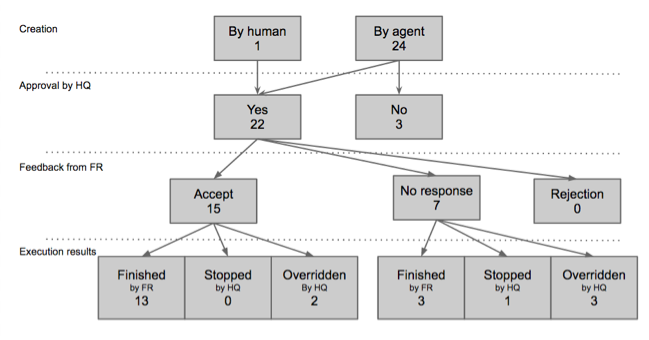
\includegraphics[width=1\textwidth]{img/study3/TaskAsSession1}
\caption{Task assignment in session 1}
\label{fig:TaskAsSession1}
\end{figure}

\begin{figure}[ht]
 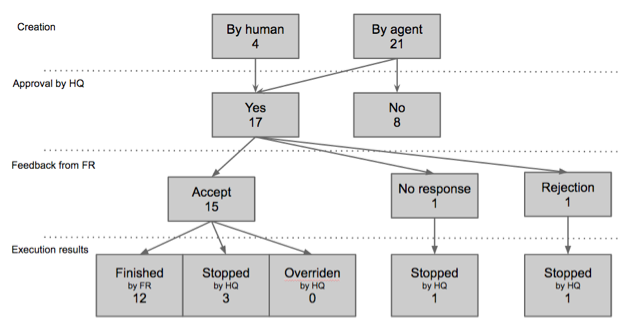
\includegraphics[width=1\textwidth]{img/study3/TaskAsSession2}
\caption{Task assignment in session 2}
\label{fig:TaskAsSession2}
\end{figure}

The summary indicates that both HQ and the planning agent contribute to the task planning activities in the control room. The planning agent created a total of 45 task assignments with additional 5 assignments created manually by HQ. HQ approved a total of 39 assignments. Field responders accepted most of the approved messages (30 out of 39). 9 assignments were rejected or not responded. During the task execution, occasional HQ interventions result in 5 task cancellations and 5 assignments override. In the end, players managed to evacuate a total of 28 (out of 40) targets in 2 sessions.\\ 

Although the diagrams (figure \ref{fig:TaskAsSession1}, \ref{fig:TaskAsSession2}) show a sequential planning-execution process (creation->approval->feedback->execution), we actually found that various planning activities (e.g. assignment creation, approval, intervention, communication) are highly intertwined in the control room setting. In the rest of the section, episodes of game play will be used to unpack the interactions surrounding the task assignment activities in the control room.\\

In the episodes presented in the following sections, players will be uniquely identified by their initials. Targets are denoted by their unique numeric target id. Task assignments from the agent are represented as two initials and one target id connected by a rightward arrow. For example, the notation PC, CR -> 22 means player PC and CR are instructed to team up and go for target 22. A standard orthographic notation is complemented by timestamps [0:00], and System Message from remote players and HQ. The HQ players will be denoted by HQ1 and HQ2. HQ1 refers to the player operating the task-assignment interface, while HQ2 refers to the player operating the situational-awareness interface.\\

\subsection{Confirming the plan}
As summarised above, a majority of task assignments are generated by the planning agent and approved by the HQ players. The episode 1 demonstrates a typical case of routine task planning process in control room. \\

\noindent\texttt{\textbf{Episode 3.1}
\emph{Context: HQ paid attention to a team (MV XW) who was carrying target 43 back to drop off zone 7.}\\
\textbf{16:45, HQ2:} XW and MV.\\
\textbf{16:50, HQ1:} (taking) 43. \\
\textbf{16:51, HQ2:} They should be going to drop off (zone) 7 and get 36 [Fig. 1] \\
\textbf{16:58, HQ1:} why don`t they go this way?\\
\textbf{16:49, HQ2:} tell them to go 36 afterwards.\\
\textbf{17:04, HQ1:} ok this one (refer to target 36). Do you tell them? [Fig. 2]\\
\textbf{17:05, HQ2:} Should I tell them? (Typing)\\
\textbf{17:07, HQ1:} Yeah, go for 36. Maybe After the drop off, I think then (will) get confused.\\
\textbf{17:13, HQ2:} I will tell them to go after drop off.\\
\textbf{17:14, HQ1:} Yeah, Yeah. \\
\textbf{18.10,} (The team dropped off target 43)\\
\textbf{18:22, HQ1:} (click re-plan) \\
\textbf{18:26,} (new assignments, the team is assigned to MV,XW -> 36)\\
\textbf{18.28, HQ1} 36, yes (Click confirm)\\
}

At the beginning of this episode, the team MV, XW are carrying a target (43), approaching drop off zone. At [16:45], the HQ2 noticed the team was going complete its current task and began to consider a new target for them [16.51]. HQ2 proposes that 36 should be prioritized [Fig. 1]. HQ1 agreed with the suggestion and decided to send the assignment after the team completes existing task [Fig. 2][17:07]. At 18:10, the team dropped off target. After the drop-off, the HQ requested a re-plan. The agent assigns the team MV, XW to target 36, which is consistent with decision of the HQ players. At the end, HQ approved the assignment [18:28]. In this typical case of task assignment, HQ  can be seen to be monitoring the task execution, and making timely requests for new task assignments. HQ`s discussion suggested that the agent task assignment was approved after a careful review of player, target and radiation status. In addition, much of HQ1 and HQ2`s discussion happens before the team drops off the target; this kind of forward planning was observed on several occasions.\\

\subsection{Just Following the Plan}
Episode 2 gives a more problematic example of accepting the planning agent`s task assignments. Episode 2.1 describes the interaction in the control room; while episode 2.2 gives the perspective of the field players.\\

\noindent\texttt{\textbf{08:32, Episode 3.2-1}\\
\emph{NG and YI have just completed a task together; DI is some distance away.}\\
\textbf{08:32,} (HQ1 request assignment for Idle player NG, YI))\\
\textbf{08:37,} (New assignment NG, YI -> 50) \\
\textbf{08:40,} (HQ1 confirmed plan) \\
\textbf{09:09,} (HQ1 request assignment for DI who has just become idle) \\
\emph{(NG have not confirmed the previous assignment; DI is closer to target 50)}\\
\textbf{09:16,} (New assignment arrived NG, DI -> 50 )\\
\textbf{09:17,} (HQ1 confirm NG, DI -> 50)\\
}

In this episode, the HQ1 request assignment twice for idle players, which is a routine activity for HQ1 (As discussed in episode 1). Firstly, HQ1 request and approve new assignment for NG, YI [08:32]. 30 seconds later, DI become idle [09:09], so HQ1 request plan again. Because DI is closer to target 50 and NG YI have not accepted their assignment, the agent replaces DI with NG in the new assignment to minimize travelling distance of field players. Although HQ1 does not verbalize his reasoning process the quick approval suggests HQ1 may not have inspected the new assignment carefully and may not have noticed that the pre- vious assignment will be overridden, potentially interrupting a task in progress. The episode 3.2-2 picks up the activity of NG and YI as the second task assignment is approved by HQ.\\

\noindent\texttt{\textbf{Episode 3.2-2}\\
\emph{NG YI received a task update after they finished their previous task}\\
\emph{(Team NG YI received new task NG, YI -> 50)}\\
\textbf{08:39, NG: } Task changed, to what? \\
\textbf{08.43, NG: } Oh sh*t, there is a radiation zone sh*t. \\
\textbf{08:53, NG: } It (target 50) is close to the lake. It is triumph road we have to go that way. \\
\textbf{08:55, YI: } Yea, we need to. No this is the lake. \\
\textbf{09:00, NG: } Oh that is the river, so it is that way, Can we go? Yes we can go, this road?\\
\textbf{09:10, YI: } Yes it should be. \\
\emph{(Their task is interrupted by new assignment YI, DI -> 50)}
\textbf{09:18, YI: } Task changed.\\
\textbf{09:19, NG: } Task changed? What? \\
\textbf{09:23, YI: } No, it is the same.  \\
\textbf{09:26, NG: } I do not see anything. \\
\textbf{09:28, YI: } You are DI, right?\\
\textbf{09:29, NG: } No.\\
\textbf{09:30, YI: } En? You are no DI? DI, wait. \\
\textbf{09:37, NG: } I can not see my Task.\\
\textbf{09:45, YI: } You are NG, Oh no, I need DI.  \\
\textbf{09:48, NG: } You should go back then. Or send a message, Oh I can not see my task.\\
\textbf{10:02, NG: } I think the page is not loading.\\
}
 
NG and YI have already received the task to rescue target 50 but have not accepted or rejected it. While they are discussing how to reach the target the second task assignment arrives [09:10], the agent requires YI to team up with the remote player DI to pursue the same target, 50. The team is confused after the change of task. YI thinks that the task did not change because the target is still 50 [09:23, YI: No, it is the same.], and NG thought the interface is no longer working [10:02, NG: I think the page is not loading.]. After YI confirms NG`s initials, she realized she needs to switch teammate (to DI). \\

Overall, the task interrupt resulted in a problematic sense making process in the field. Meanwhile the players in the control room appear unaware that anything untoward has occurred. The observation also reveals that several factors could have led to the task interruption including the absent of response from field responders; computational planning performed by agent without timely field feedback; and HQ`s failure to discover the task interruption during assignment approval. 

%This episode can be an example showing that computationally `optimized' assignment is not socially optimized for teams and HQ supervision failed to tackle the issue.\\

\subsection{Correcting the plan}
HQ players occasionally chose to change the task assign- ments generated by the planning agent; episode 3 presents one such example.\\

\noindent\texttt{\textbf{Episode 3.3}\\
\emph{CE and KH are currently assigned target 03 but have not accepted; other players are free}
\textbf{04:18,} (HQ1 click request plan)\\
\emph{(Assignments arrived: CE KH -> 06, MP GO ->07, MB ,WB -> 10)}\\
\textbf{04:24, HQ1:}  What? Why I am getting? Ahh, one of these guys does not accept. [Fig 7] \\
\emph{(Referring to the team of CE, KH.)}\\
\textbf{04:29,} (HQ1 clicked keep on assignment CE KH -> 03) \\
\textbf{04:33,} (HQ1 request re-plan)\\
\textbf{04:40,} (Assignment arrived: MB, WB -> 10, MP, GO -> 07)\\
\textbf{04:42,} (HQ1 click confirm)\\
\textbf{04:56,} (MP, GO accepted)\\
}


After HQ requests a new plan, agent proposes a set of assignments, one of which (CE KH -> 06) interrupts existing task of a team (CE KH -> 03). HQ1 queries this change (``What? Why I am getting?'') realises that they have not explicitly accepted the previous task [04:24]. It should be noted that this kind of task interruption only happens when field players did not accept the tasks (Section \ref{sec:study3system}), making agent think they are idle at that moment. After finding this problem, HQ then requires the agent to ``keep'' existing assignment [04:29] and requests a new plan from the agent, which is then approved. In contrast to episode 3.2, HQ1 notices and compensates for the field players` failure to explicitly accept the task, and the field players are able to continue with the previously allocated task without interruption.\\

\subsection{Changing the plan}
At the start of session 2 there is an extreme example of the HQ players overriding the planning agent. \\

\noindent\texttt{\textbf{Episode 3.4}\\
\emph{Context: At start of the session 1, all players were idle waiting for initial plan.}\\
\textbf{01:25,} (HQ1 requested initial plan)\\
\textbf{01:28,} (4 initial assignments arrived) [Fig 3] \\
\textbf{01:29, HQ1:}  why, it is stupid. \\
\textbf{01:33,} (HQ1 click edit)\\
\textbf{01:53, HQ1:} I want this one (HQ1 drag target x to replace agent planning, see Fig.4) this one and this one.\\
\emph{HQ1 replaced 3 out of 4 targets in the task assignment. The three prioritized targets very are close to the original cloud}\\
\textbf{02:03,} (HQ1 clicked confirm) [Fig 4]\\
\textbf{02:07, (HQ1 talk to HQ2) HQ1:} I think we should get the far ones first. \\
}

The episode begins with HQ requesting initial task assignments for the whole team. When the agent gives HQ  a set task assignments for approval, HQ complained about it [01:29, HQ: why, it is stupid.], indicating he is not satisfied with the plan. HQ then click edit button to switch to edit mode. Under the edit mode, HQ dragged 3 targets to replace the targets in agent assignments. The three prioritized targets are the ones that are closet to the radiation cloud [fig 3]. After HQ confirmed his modification [02:03], he said to HQ2 that the far away targets should be rescued first [02:07]. The execution result of this heavily edited plan is not ideal. Among the 3 three modified assignments, 1 finished 1 assigment is cancelled later, 1 assignment leads to player death.\\

\subsection{Coping with the unexpected}
Episode 3.5 picks up shortly after episode 3.4, which exemplifies how HQ adapts task assignments to changing task status. \\

\noindent\texttt{\textbf{Episoe 3.5}
\emph{Context: At start of the session 1, all players were idle waiting for initial plan.}\\
\textbf{02:09, HQ2:} they cannot walk there straight. [Fig 5]\\
\emph{Referring to team MB, GO, HQ2 point out that the straight path to one of the target is blocked by radiation}\\
\textbf{02:14, HQ1:} So who is that. (Target) 04 (HQ1 open the message panel) \\
\textbf{02:20, (HQ 1 Types message)}  You are heading to an area affected by cloud, You need to be very fast. [Fig 6] \\
\textbf{02:45, HQ2:} 04 is now in the cloud. \\
\textbf{02:45, HQ2:} Oh god, that is so fast.\\
\textbf{03:20, (HQ1 Types message)} Stay to the lake as possible!\\
\textbf{03:33, HQ1:} Shall we cancel (assignment 04) that or shall we wait for report? (HQ1 opens msg panel to talk to MP GO)\\
\textbf{03:43,} (HQ1 opens msg panel to talk to MP GO) \\
\textbf{03:50, HQ2:} I think (Target) 04 is only an animal, screw the animal.  \\
\textbf{03:52, (HQ1 Types message)} Abort, target compromised, proceed to target 07. \\
\textbf{04:06, } (HQ1 sent message)\\
\textbf{04:11, } (HQ1 click stop on the assignment of MB, GO->04)\\
}

After confirming assignments in Episode 1, the HQ2 point out one assignment may be impractical because the route to target has already been blocked by a radiation cloud [02:09] [Fig. 5]. HQ immediately open message panel to send warnings and urging the team to move fast [Fig. 6]. However the cloud expansion seems to be faster then HQ originally expected [02:51]. Apart from sending route guidance in the team, HQ started to consider cancellation of the assignment. After HQ2 agree with the cancellation, HQ send a message to the team to inform them the assignment is going to be cancelled and instruct them to go to new target 07. The assignment is formally cancelled in [04:11]. After HQ1 cancelled the task, he started to request new assignments from planner and allocated target 07 to the team later. In this case the HQ players realise the risk and are able to abort the task and redirect these field players out of danger.\\

\subsection{When it all Breaks Down} \label{sec:playerDeath}
In the episode 3.5, in which the HQ modified 3 agent assignments. In the modified plan, the team CE, KM is instructed to go for a target very close to a radiation cloud. We look first at the HQ perspective (episode 3.6-1), and then at the field players` perspective (episode 3.6-2).\\

\noindent\texttt{\textbf{Episode 3.6-1}\\
\emph{(Context: One team (CE, KM) is end up heading to radiation cloud. )}\\
\textbf{4:52, HQ2 } They (CE KM) are walking right into their death. \\
\emph{(CE and KM were heading to target 03 which is now at opposite side of a radiation cloud)}\\
\textbf{5:14, (HQ messaging) } Careful, you are approaching the cloud. Move extremely fast to the cloud. Go around the lake to return.\\
\textbf{5:32, HQ: } God, too slow.\\
\emph{(The team CE KM is completely in the mid of radiation)}\\
\textbf{5.46, (HQ typing message) } Move closer to the lake.\\
\textbf{5:50, } (The team went through the cloud, their health is below 20, the target 03 is now at the edge of the cloud)\\
\textbf{6.39, HQ2: } What are they trying to pick up?\\
\textbf{6:43, HQ1: } The fuel.\\
\textbf{6.48, HQ2: } I am not sure whether they can survive picking up the fuel. No, now is more concern of surviving. \\
\textbf{7:05, (HQ messaging) } Abort 03, return top to (target) 99. \\
\textbf{9.04, } (HQ1 stopped task of CE KM) \\
\textbf{9.05-10:08, } (HQ requested re-plan 4 times, no new plan available for CE KM) \\
\textbf{9.50, HQ1: } No targets for them? There are lots of them. \\
(Team CE, KM stay in the cloud all the time, and finally dead)\\
}

At the beginning of the task, the radiation cloud has already between target and the field team CE and KM. The cloud was expanding quickly, which caught the HQ1 in surprise. As a result, 2 messages were sent by HQ1 to guide the team to avoid the cloud [05:14,5:46]. However the team was still excessively exposed to the radiation when they reached the side of the target, so HQ1 decide to abort the task [07:05]. After HQ1 cancels the assignment, the team is still exposed to radiation. HQ1 then tries to assign the players to other targets by requesting agent for new assignment [09:05-10:08]. However, the agent does not assign the team to any task because the team`s health is too low. HQ1 seems to be confused about why the agent refused to assign targets. He continuously requested plans for three times and said ``No targets for them? There are lots of them (refer to targets).''[9:50] During this process, the team was still standing in the cloud. They finally lost all the health points and become incapacitated. Field player`s perspective is given below. \\


\noindent\texttt{\textbf{Episode 3.6-2 }\\
\emph{CE and KM are heading towards target 03}\\
\textbf{05:15, CE: } (Reading out the message) You are approaching the cloud, move extremely fast to the cloud, Ok! \\
\textbf{05:21,} (CE grabbed KM and started running) [Fig 8]\\
\textbf{06:12,} (The team CW, KM ran all the way across the cloud) \\
\emph{(After ran through the cloud, they are checking the health value.)}\\
\textbf{07:02, CE: } how dead are you?\\
\textbf{07:04, KM: } Pretty much dead.\\
\textbf{07:06, CE: } I am pretty dead as well.\\
\emph{(The team is trying to locate the target, but it is unsuccessful) [Fig, 9]}\\
\textbf{07:28, CE: } Do you know what is funny? We have to get back.\\
\textbf{08:24, CE: } It should be somewhere around here! We are getting close.\\
\emph{(Assignment cancelled)}\\
\textbf{08:52, CE: } there is a new task, No task at the moment? \\
\textbf{[...]} 
\emph{(After assignment was cancelled, the team was still trying to locate the target)}\\
\textbf{09:44, CE: } I am pretty much dead and radiation is 12. Where is it! It says it is on this street but it is not. \\
\textbf{10:06, CE: } Oh I am dead.\\
}


The part 2 began with player CE reading the HQ message (``You are approaching the cloud, move extremely fast''). After this message, CE grabbed teammate KM and starts to run through the cloud [Fig. 8].  After they ran through the cloud, the team check their remaining health value [07:02] and started searching for the target at the edge of the radiation cloud. About half minute later, the assignment is cancelled by HQ [08.52] and no further task is allocated (as seen above). Although the task has been cancelled, the HQ failed to assign new task to the team [3.6-1, 9:50] . The field players note but then appear to ignore HQ1`s in- struction to abort [08:24] and continues to search for the tar- get. The field players seem to interpret the lack of a new task as license to remain where they are and are eventually overwhelmed by the radiation.\\

\subsection{Missing feedbacks from field}
Lack of feedback leads to false assumptions of the agent (players are still available), which in turn compromises its optimization (Section x). we also found that HQ may also be distracted by the lack of response, in that they have to guess player`s intention without their feedback. \\

\noindent\texttt{\textbf{Episode 3.7}\\
\emph{(New assignment MV XW -> 36, XW accepted, MV had no response)}\\
\textbf{13:05: HQ1: } I think they have not received any task probably . \\
\textbf{13:22, HQ1: } Just do not have response, I do not know why.  \\
\textbf{13.32, HQ2: } MV and XW, I suppose they go to 36. \\
\textbf{13:35, HQ: } They are moving, but they did not accept that. \\
\textbf{13:48, } (HQ click request, new assignment to MV XW -> 43, NO response from MV XW)?\\
\textbf{13:51, HQ2: } I am not sure they are still going south; I think they (MV XW) are going to 43 instead. \\
\textbf{13:59, HQ1: } HQ: they are going to 43.\\
\textbf{14:05, HQ1: } HQ: they just do not have any response, no reply. But they are coming for it, they are coming. \\
}

In this episode, the team MV, XW was assigned target twice [12:30,13:48], but the team neither rejects nor accepts those two assignments. The HQs are observed to guess intentions of the field responders 3 times [see 13:32, 13:51,13:59] and complain about the non-response twice [see 13:22, 13:48]

\subsection{Division of labour in HQ}

In session 1, the responsibility for HQ1 and HQ2 to send messages are not fixed as original design, but dynamically negotiated between the two HQ operators. The following fragment is a typical case of the negotiations.\\

\noindent\texttt{\textbf{Episode 3.8 }
\textbf{17:04, HQ1: } Ok this one (refer to target 36). Do you tell them? \\
\textbf{17:05, HQ2: } Should I tell them? \\
\textbf{17:07, HQ1: } Yeah, (tell them to) go for 36. \\
\textbf{(HQ2 sent message) } MV and XW  move north of the water and go round to 36\\
}

In this fragment, HQ1 asks HQ2 to send a message to instruct a team to go for a target 36. The message is a task-specific, but it is sent by HQ2 through the broadcasting message channel.\\

In session 2, we do not find similar negotiations. However, in the post game discussion, the HQ2 expressed that he has too little to things to do (other then sending general messages), while HQ1 has too much to do:\\

``The interface I use was completely useless, became I can only message everyone at the same time, basically spamming everybody, so the only thing that I can do is, Oh , the cloud moves there and there. At the same time, Khaled (HQ1) had to message to everybody privately. While he was doing that, he coundn`t do new plans. So there is a lot stuff for him be I coundn`t do anything.''\\

\section{Discussion}\label{sec:study3discussion}

In previous section, episodes are presented to illustrate how the In-the-loop interaction design plays out in the field.  The episodes reveal that, to large extent, human the HQ players are successfully involved in the control loop. However, we also found some confusions and misunderstandings occur between agent and human which may leads to issues and implications for interaction design.  \\

\subsection{How does the In-the-loop design play out?}
The interface functionalities are designed to enable HQ to engage in arrange of interface interactions such as plan requesting, editing, approval and cancellation. This section exams how these functionalities are utilized and to what extent do they help HQ stay in the control loop. In what follows, we firstly examine the usage of individual interface functionalities. Combining the episodes presented in previous section, we then, reveal how the division of labour plays out with support of these interface functionalities.  \\

\begin{enumerate}
\item \textbf{ Plan request and approval } The plan request function is used by HQ to trigger the agent re-planning. The design of the plan approval stage gives HQ an opportunity moment to review and influence the final plans before it is sent to field responders. Both functions are essential for human and agent to collectively produce task assignment, constituting the routine task planning work in control room. The two functions are the two most frequently used interface functionalities (HQ requested plans for 45 times; approved 39 task assignments). Deciding appropriate moment to request plan and approve desired assignments require HQ to closely monitor the task status. The uses of the two interface functionalities are usually observed together with discussion of task execution status, which indicates HQs are engaged in the planning-execution loop with a supervisory role. \\

\item \textbf{ Plan edits } The ``plan edits'' enables HQs to directly intervene the planning. We observed HQ`s modified undesirable agent plans twice throughout the field study (Episode 3.3, 3.4). It should be noted that the function is designed to be used infrequently, because the planning agent is supposed to take over the majority of the computational intensive planning activities. \\

\item \textbf{ Plan cancellation } Further, the task cancellation functionality allows HQ to influence task execution after the plan approval. In episode 3.5, we observed assignment being cancelled and teams being reassigned due to unexpected cloud activities. This may suggests that combination of cancellation and re-planning can be a useful tool for HQ to respond to contingencies in the task execution.\\

\item \textbf{ Partial planning } The partial planning functionality allows HQ`s to indirectly influence on the planner. For example in episode 3.3, HQ identified task interruption in proposed plan. He then required the agent to keep an existing assignment and perform re-planning again.  This episode can be seen as a case in which HQ is able to make sense of the task status and utilize the partial planning functionality to influence the assumption of the planner agent. \\

\end{enumerate}

Apart from the above mentioned functionalities to support HQ intervention, the task assignment interface appears in many cases to provide an effective shared representation of the current state of the game. As well as showing current player and target locations and player health it also makes visible the currently approved task allocations, field player responses and any new plan that has been requested or is being edited. This shared information forms the common ground between the HQ players and the planning agent.\\

HQ players are observed to closely monitor this view and its representation of plan execution. For example episodes 3.1, 3.2, 3.3, 3.5 and 3.6 all reveal HQ players` awareness of field player progress and current tasks, episodes 5 and 6 show awareness of the cloud`s location in relation to players, and episodes 3.1, 3.3 and 3.4 show HQ players engaging actively with proposed (rather than current) task assignments. We observe that the HQ players are quite capable of modifying the agent`s plans when they wish to, for better (episode 3.3) or worse (episode 3.4). HQ is also able to intervene in current task allocations, which is successful in resolving the situation in episode 3.5 (but not in episode 3.6).\\

%The usage of individual interface functionalities indicates the interface functionalities may actually serve its design purpose, which is to support the HQ requesting, editing, approving and cancelling the plans. In what follows, we will examine how the division of labour play out as a result of the interface support. the observation reveals that HQ players contribute to the planning with a set of supervisory activities, while the agent take over computational optimization of task allocation. \\

%1) Firstly, HQ players are observed to closely monitor the plan execution. For example in Ep 1, field players` task progress is mentioned by the HQs. In episode 3, HQs expressed their concerns about cloud and player locations, while in episode 6, HQ`s are more concerned with the uncertainty of field players` intention. The task \\

%2) Occasionally, HQs also need to modify plans when agent proposed plan is not desirable. For instance in Ep 2, HQ overridden 3 our of 4 agent proposed assignments to implement his own strategy. Further, HQ`s intervention is also required when contingency rises from task execution. For example, The HQ terminated an approved assignment due to unexpected cloud activities. A re-plan is quickly followed up to assign new assignments to the affected teams.\\ 

%3) The forward planning activities are occasionally observed. For example, HQ`s discussion of future plans for a team is observed in Episode 1. The forward planning activity is thought to be not well supported by the system and it is unclear whether this activity contributes to the planning. More details will be discussed in section x. 

On the other hand, the agent is found to take over computationally complicated task optimization, freeing up the HQ to play their supervisory roles. Throughout the two sessions, the HQ requested the planner to re-plan for 49 times. The agent generated 45 task assignments, 34 out of which are approved by Headquarters. In comparison with the agent planner, Human only created 5 task assignments. The fact that agent creates large proportion of assignments suggests the agent successfully takes over the routine planning to a large extent. \\

In many cases the communication between HQ and the field players is unproblematic, and most targets are successfully evacuated according to plan. This situation seems to be considerably better than that reported in Chapter \ref{ch:studyone} and Chapter \ref{ch:studytwo}, and we conjecture that this is due at least in part to differences in the mobile interface in the trials reported here. Specifically, unlike in the studies reported there, the current task allocation is shown as a graphical overlay on the mobile map, not just as a textual instruction (given by the HQ player in Chapter \ref{ch:studyone} or the planning agent in \ref{ch:studytwo}). This seems to significantly reduce the field players` confusion about their current target and team- mate and where to find them. The seemingly better situation of task communication is consistent with the requirement (Section \ref{sec:study3system}) outlined for interface improvement that stresses the importance of structured, domain-specific task representation for both HQ and field responders.  \\

A pattern of labour division is also observed between the two HQ players in control room. To recap, the two HQ players in control room are split into two roles. The role of HQ1 is responsible for handle task assignment and send assignment-specific messages to field responders. The role of HQ2 is to support monitoring task status and send general chat messages. As a result, the messaging system of the messaging is split in to two channels (general information and assignment-specific, Section \ref{sec:study3system}). The messaging interface allows each HQ player to take control of one of the messaging channel. This designed role division is briefed participants in training session before the game play. However, the system does not play out as designed in the field study. 11 messages in the general message channel are task specific, which indicate the HQ players may occasionally violate the designed division of responsibility. As we have seen, in session 2 the HQ players accepted this division of capabilities but were frustreated by it. However in session 1 the HQ players developed their own work-arounds for this based pn verbal negotiation, so that at times HQ2 would use the general broadcast interface to send task-specific messages for HQ1, relying on the identification of the intended field players by their codes within those messages.


\subsection{Responsibility and Complacency}\label{sec:huilimperfection}
In the game probe, the planning can be seen as partially automated by the planner agent. The task optimization performed by agent is thought to be `imperfect` because it fails to consider any organizational efforts/overhead required execute the plans and plan changes, that is, the social cost of implementing plans. The result of this imperfection has been exemplified in previous chapter (Chapter \ref{ch:studytwo}), and also Episode 3.2 and 3.3. In the episodes 3.2 and 3.3, it proposes new plans that will disrupt ongoing activities, albeit because the respective field players have not (yet) explicitly signalled their acceptance of these tasks.\\

The imperfections are thought to be ``natural'' for agent planning support, as computationally ``optimized'' assignments from the planner may not socially optimized for the responder teams (Section \ref{sec:study2social}). It highlights the importance of human involvement in the planning activities. In principle, the human in-the-loop interaction design allows the human, in this case the HQ players, to take active responsibility for system. For example, in episode 3.3 we see HQ1 successfully `correcting' the plan to allow for missing information (responses) from the field players. However in episode 3.2 the HQ player failed to prevent the unnecessary task interruption in the approval stage, resulting in extra coordination work and sense making for field responders. Considering this case in more detail we see that it arose from the combination of: lack of field player feedback; failure of HQ monitoring; and the particular computational optimization performed by agent (which assumes that there can be no overhead if a task has not been formally accepted).\\

The failure case in the episode is similar to the well-observed phenomena discovered by automation researchers called complacency \cite{Kaber1997}. The complacency phenomenon refers to the human failure of detecting occasional automation failure. Study of automation suggests that complacency can be classified as attention-based monitoring failure, which is likely to happen when human is engaged in multi-thread tasking. In the case of episode 3.2, the quick approval of problematic assignments suggests the plan is not properly reviewed. The HQ`s attention could be a factor of the monitoring failure. As the HQ player is trying to allocate tasks for idle players, they may exclusively focus on the new assignments for the idle players rather then other conflicting assignments.  If the interface failed to attract HQ`s attention to the conflict, HQ may approve the plan as long as idle players are properly assigned. Although failed in episode 3.2, the interface highlight does grabbed attention of the HQ in episode 3.3. Some study shows that complacency is found in both naive and expert participants and cannot be overcome with simple practice \cite{Parasuraman2010}. Therefore other mechanisms to counter the complacency effect may be needed, such as a richer involvement of the human in the planning, which we pick up further in Section \ref{sec:study3supportPlanning}.\\

\subsection{Tacit confusions}
While many interactions were essentially unproblematic we do observe a number of areas where silent, missing or invisible information led to confusion and break down.\\

For field players, the task cancellation is presented a notification (``task changed'') followed by a blank task page only with the text (``No task assigned at the moment''). The field study suggests the presentation could be problematic for the field players. Firstly, being assigned with no task does not successfully convey the meaning task cancellation (``Don`t carry on''). The episode 3.6-2 (part 2) shows a case in which the players completely ignores the task cancellation and carry on doing and risky task. In episode 3.2-2 (part 2), the player NG even think the blank task interface implies malfunctionality of the mobile interface. Even if the players understand task cancellation, its implication can vary. Without a task, the players can chose to, for example, (1) stand by doing nothing, (2) find targets by themselves, (3) escape for life. Therefore, the field players may be confused about what to do next. In another example (not presented) of cancellation, the field players were stuck in a radiation cloud when their task was cancelled. With high radiation reading and loss of target, they don`t know what to do next so they send messages to HQ for clarification. They finally left the radiation cloud after they receive and accept new assignments from HQ. This example shows the implicit instruction of ``DON`T CARRY ON'' is confusing. Instead, the explicit instructions, which directly point out what to do next may be desirable. For example, in the case of AtomicOrchid, frequent instructions can be ``stand by'', ``reverse back'' and ``escape''. We therefore argue that interface should encourage HQ consider such ``explicit'' instructions and support quickly sending such instructions. \\

Second, episode 3.4 in which the HQ player drastically modifies the agent`s proposed plan illustrates vividly that the current interface makes the agent`s proposed plan available to the HQ player, but does not reveal the agent`s priorities or reasoning. The HQ player enacts a policy of evacuating the targets nearest to the radiation cloud first, presumably in the belief that the planning agent has (a) used a different priority and/or (b) not given due consideration to evacuating those targets. In fact the planning agent will have considered and rejected those targets, based on its model of field player movement, radiation cloud spread and `permitted' radiation exposure (none). None of the agent`s models are likely to be perfect but at present they are not open to inspection. It soon transpires (episodes 3.5 and 3.6) that the HQ player`s initial expectation of how quickly the radiation cloud will spread is very wrong. In an ideal world we would want this information to be available to the HQ players, so that the common ground can be expanded to include not only the plan but the reasoning behind the plan. However, as in the previous point, there is also the challenge that we may overwhelm the HQ player with information in a time-critical decision-making situation.\\
	 
Apart from the issues of task cancellation, the issues of field player feedback also emerged. The field observation showed that the feedback system is crucial for both agent and HQ players to keep track of the task status. Overall, most of (30 out of 39) the assigments have been responded by the field players. However, there are still a number of un-responded assignments that causes issues in coordination. For agent planner, the lack of field response may lead to false assumption of availability of the players, which in turn, compromises the subsequent re-planning (Episode 3.2 and 3.3). For the HQ players, the lack of field response adds to the uncertainties in the task status as well. HQ players have to take efforts to guess the intentions (Episode 3.7). We might wish that the field players would always respond in a timely manner. However there may be good reasons why they have not or cannot at present, e.g. if they are incapacitated or there are temporary problems with communication. Also, in the scenario of AtomicOrchid, no matter how fast the responders accept assignments agent planning may happen concurrently.\\

One strategy to view the issue of field response is to treat the lack of response as an uncertainty in the task execution, and it might be better for the system and agent to view this lack of information more positively and concretely as a `known unknown'. For example, the planning agent might create a plan (or multiple plans) that take into account the possibility that these assignments may transpire to have been accepted or rejected (at least in the player`s thoughts). Similarly, the interface might make visible the uncertainty, and perhaps also highlight the other information which could be impacted as a result, such as contingent plans. \\

Interactive system researchers have outlined a list of strategies to tackle the inevitable uncertainties, one of which is to reveal the uncertainties to operators so that they can make informed decisions \cite{Benford2006} \cite{Skeels2008}. One straightforward approach for visualizing the uncertainties is to highlight the affected data. Methods for highlighting have been proposed in literature \cite{Conti2006}. However, in the real-time control scenario like AtomicOrchid, the highlighting approach has to be applied with caution.  The operators have limited resources (attention, limited time and cognitive workload capacity) to tackle various issues in a multi threading, time constrained task setting. Abuse of interface highlighting may contend for the limited resources. There are evidences showing that, visualization of uncertainties is likely to overload decision makers in time limited decision-making, which in turn, degrade their ability to respond in a timely manner \cite{Zuk2007}. Take episode 5 as example, although the system highlighted potential task interruptions as a result of lack of response, operator still ignored it. \\

In episode 3.6, the HQ  become confused when the planner stop giving back assignments. In this case, the HQ repeated requesting plans four times and complains about no response from planner. However, the planner does not produce more assignments simply because the idle players have little health to take any more assignments. This policy and reasoning of agent planning is not visible to the HQ player (although in this case the reasoning leads to not doing something, which may have its own representational challenges). \\

\subsection{Support human planning} \label{sec:study3supportPlanning}
%positive bit
As seen in all episodes, HQ players are observed to utilise the task interface to assess current game status, while in episodes 3.3, 3.4, 3.5 and 3.6 we have also seen how they can modify the agent`s plans. This suggests that the interface is sufficient in providing basic situational awareness for HQ players to make their own plans. The drag-and-drop based plan editing interface also enforces various constraints on task assignment so that all plans are at least valid, i.e. well-formed. For example, each player and each target can be assigned to at most one task, and each task can only have players with the correct combinations of game roles for the target. The interface also highlights players and targets on the map when they are manipulated so that the HQ player can readily assess location and proximity when editing task assignments. In the view of situated actions \cite{Suchman1987}, the plans for the team is itself a projective representation of actions. What the system achieved here is to enhance the representation on the interface level and open an opportunity for human teams to sketch on the representation with situational awareness support. However, the observations also reveal some potential for improving support for human planning.\\

Returning to episode 4, the HQ player massively revises the plan. The modified plan turned out to be undesirable as it leads to 2 assignment cancellations and 2 player deaths (Episode 3.6).  We observe that the planning agent is silent with regard to the problems in the player`s proposed plan. As the planner has ruled out the risky plan at the first place, the reasoning behind the original plan may be important information that should have been exposed to HQ to inform their decisions. While making visible the planning agent`s reasoning might have discouraged the player from changing the plan so dramatically, there will still surely be situations in which plans could or should be changed. And in this case the player is currently left to ``do their best''; in short, the current system will make plans for a person to change or approve, but will not help that person to plan beyond ensuring that their plan is well-formed. If, rather, the planning agent were to simulate (and perhaps extend) the proposed modified plan then it could provide the HQ player with at least one view of the possible outworking of their plan.\\

In the current system the agent performs forward planning, i.e. it considers what field players might do in the future, not just in the current/next task assignments. However this in- formation is also not made available to the HQ players. In episode 3.1 we also saw one of several examples of the HQ players also planning for future task assignments. However they had no way to record this or feed it into the system; they simply had to make a note or remember what they were thinking when the current task was completed and they had the chance to check and intervene. For at least some situations it might offer benefits if the agent`s future plans could also be viewed, and if the HQ players also had some way to support their own future thinking.\\

However, again we are considering attempting to visualise and interact with significantly more data and more complex data which is liable to further complicate the interface. For example, for the agent to share information of its reasoning behind a particular task assignment, it may need to present its prediction of the future game status and its assessment of current game status. It may well be problematic for HQ to digest this extra information in a time-constrained task environment. Various studies have identified the problem of information overload in the system interaction design in disaster management domain \cite{Carver2007}, \cite{Turoff2004a}. The problem occurs when information presented at a rate too fast for a person to process \cite{Hiltz1985}, and it may lead to a list of human performance consequence \cite{Hiltz1985}:\\

\begin{enumerate}
\item Fail to respond to certain inputs,
\item Respond less accurately than they would otherwise,
\item Respond incorrectly,
\item Store inputs and then respond to them as time permitted,
\item Systematically ignore (i.e., filter) some features of the input,
\item Recode the inputs in a more compact or effective form, or quit (in extreme cases).
\end{enumerate}

Various techniques have been explored to alleviate the problem of information overload in different application domains such as security monitoring \cite{Conti2006}, teleoperation \cite{Kadous2006}, and communication systems \cite{Hiltz1985}. However, the specific research of information overload for task allocation support in DR domain is still rare. We think that the extra forward planning support may introduce the risk of overloading human operators. Therefore, more studies are required to evaluate the trade-off between its benefits and consequences for human performance.\\



% \subsection{Unsupported forward planning activities} merge
%The agent performs n-step [need to confirm] looking ahead planning (see section of agent algorithm) for each re-plan. Similar to the agent, HQ players are observed to engage in forward planning activities. For example, in Ep 1, the HQ anticipated a team was going to finish assignment soon and plan to assign a new target for them. Later, HQ triggered a re-plan and the result was consistent with the HQ`s previous plan. In some other cases, the result of agent re-planning was not consistent with HQ`s plan. Therefore, HQ has to make decisions about whether to follow the agent or not. As both HQ players and the agent conducted forward planning, sharing of relevant information may help HQ to understand the agent`s reasoning and make informed decisions.  Again, excessive and ineffective explanation of agent plans may introduce the danger of overloading the HQ players.  [Connecting to information overload]




%7.* Smoothing the workflow\\

%8.* Accountability become opaque by using the agent. \\

%[a separate reading list available for this chapter]\\

\section{Lessons from interaction design} 
Herein, we offer a brief summary of the lessons learnt that may benefit the designers of planning support systems, in particular, in relation to situation awareness, human error, and interacting with computational planning. These may be particularly relevant for settings in which timely human decision-making is critical. We furthermore also set our lessons into context with related work.

\subsection{Common ground}
Common ground is a critical requirement to making collaborative decisions in an effective and timely manner. Through our field trials, we identified the following features as constitutive to common ground through providing a mutual situation awareness for the participating parties (HQ, field responders, and the agent).
\begin{itemize}
\item \textbf{Shared representation}. The task interface enabled common ground between HQ players and the planning agent -- the basis for enabling HQ players to read, modify, and confirm the agent's task assignments. Shared representation was also critical to align field players and HQ view of the environment, e.g., through the messaging channel.  
\item \textbf{Awareness of current state}. Episodes evidenced HQ displayed awareness of task progress, threats, and field responders' locations and proximity as critical in their planning.  
\item \textbf{Domain-specific task representation}. Providing a consistent representation that made use of domain-specific visual cues was an important feature to enable alignment and consistency across views and between mobile (field) and stationary (HQ) representations. 
\item \textbf{Awareness of future actions}. HQ engaged with \textit{proposed} tasks -- reading proposals in conjunction with awareness of current state, modifying, and confirming was seen to be an essential aspect of the situated planning work. 
\end{itemize}

Our recommendations also align with the theoretical framework model of situation awareness proposed by \cite{Endsley2001}, which argues the SA needs to be supported by three levels including 1) Perception of the elements in the environment 2) Comprehension of the current situation and 3) Projection of future status.\\ 

\subsection{Supporting Mixed-Initiative Planning} 
Some interactional challenges have become evident in the field trial that can be attributed to the interaction with the computational agent. \\

\begin{itemize}
\item  \textbf{Constraining task assignments} was seen as a clear advantage of the planning support in this setting, to guarantee only well-formed task assignments.
\item \textbf{Making reasoning visible}. Modifications of plans as a result of which responders were sent in harm's way may have been avoided if the grounds upon which the agent computed task allocations had been available for inspection. The challenge is how to implement this without inundating the operator with information.
\item \textbf{Feedback on modifications}. As further step to making visible, the agent could also provide feedback on human modifications of its task assignments, e.g., in terms of safety and risk.
\item \textbf{Forward planning} of the agent could be made visible on demand to enable planning ahead. 
\end{itemize}

Our recommendations echo seminal work on human considerations in context-aware systems, which provided principles to support intelligibility and accountability \cite{Bellotti2001}; similarly we stress that the goal for planning support systems should be  to be accountable for their actions, therefore, `what they know, how they know it, and what they are doing about it' [ibid., p. 201] needs to be legible by the operator. Furthermore, as planning is oriented towards the future, yet produced as a contingent, situated activity \cite{Suchman1987}, the interface needs to support revision and revoking of plans in situ, and furthermore provide the situational awareness essential to do so.  

\subsection{Interactional trouble}
We have encountered the following interactional challenges that likely generalise more broadly to related settings.
\begin{itemize}

\item \textbf{Complacency} describes the phenomenon whereby occasional failures of automation may be difficult to detect \cite{Kaber1997}. Particularly, when the operator has learnt to trust the computational component. Mechanisms to counter may turn towards more human involvement in the planning, however, there will be a fine line so as not to create information overload. 
\item \textbf{Non-responsiveness} has been observed to create uncertain situations. It is important to realise this could equally be caused by technical communication outages, as well as by human non-response. Designers may attempt to incorporate this as  `known unknowns' in the system, for example planning could be done with an estimated \textit{probability} of a positive response. 
\end{itemize}   

The wealth of computational approaches to the problem of `planning under uncertainty' \cite{Chang2007} suggests uncertainty are is a key recurring problem, particularly in time critical settings. In this context, it may also be important to look towards interface design guidelines to complement computational approaches in order to avoid or minimise human error at the interface level \cite{Norman2013}.


\section{Professional feedbacks}\label{sec:RGworkshopone} 

The section will present the results of a workshop we conducted with a professional disaster response charity called Rescue Global (RG). The purpose of these workshop is to get professional feedbacks about the AtomicOrchid(AO) platform to understand realism of the disaster simulation based on AO. Based on the feedbacks, we reflects on strength, limitations and potential improvements of AO platform. \\

The workshop is centred on a demonstration of HAC-ER system for disaster response (DR) \cite{Ramchurn2015}. The AO is a component of the HACs demo system. Others components include information crowdsourcing, multi-UAV control interface for DR, and DR operation provenance store (Section \ref{sec:lraisupport}). Each component are allocated one session (about 45 mins). The AO session is structured as follows:\\

\begin{enumerate}
	\item A presentation introducing the AO platform and HQ interface.
	\item A handles-on session for RG members to operate the HQ interface. For the purpose of demo, the field players in AO are simulated.
	\item A discussion of AO platform for Rescue Global to reflect on some themes including: Command and Control structure, Division of Labour/Task and team planning.
\end{enumerate} 

We also encourages free discussions throughout the AO session, which leads to some emerged themes including: Data connection, time-scale of planning in real DR operations and other interface improvement suggestions.  

\subsection{The Rescue Global feedbacks}
Based the feedbacks from the RG, the AO setting  mirrors some aspects of the RG`s disaster operations. Firstly, the RG member quickly recognise the task-team matching mechanism is very similar to the aspects of resource-needs matching in their operation. At the beginning of the introduction presentation of AO, one of the responder commented: \\

\begin{quotation}
``This is actually very similar to what we do when we do reconnaissance now. We identify needs, and we are aware of what the resources that we have and match it into what resources we have and match the needs into resources.''\\
\end{quotation}

Further, the team formation mechanism can also be mapped to aspects of their operations by the RG members.The RG confirmed that members from different organisations and different skills often teamed together for tasks. However, the cross-organisation teaming activities are mostly done in an informal way, as one RG members described: \\

\begin{quotation}
``What we did in Philippine is that , say we found school, and we talked to the MSF medics we have bumped into. They have medics, can run some clinics there. Then they need some security, they are comfortable with Simon and Bren (two path finder in RG), we can help them out, we did that, but almost informal way'' \\
\end{quotation}

The statements of RG indicates that their collaboration with the MFS medic teams are based on informal  relationship with them and the formal organisational collaboration is often missing. The RG also stressed that the paradigm of cross-organisation team formation in AO is desirable, but difficult to achieve in a formal way.They highlighted the major challenge for realising AO paradigm is organisational. As the one RG member stated:\\

\begin{quotation}
``The challenge with that is that UN clustering system, make separation of different tasks, they then delegate the tasks down to say Health cluster, and UNISAF, all the way to little agencies, they won't work with anyone else, because they do not know them, they do not have relationship, so UN structure stops that... does not mean you can not change it, but current paradigm would not allow it ''
\end{quotation}

Based on RG's feedback, we also identifies some unrealistic aspects of AO setting. Firstly, RG member expressed the concerns related to data connection. They highlighted that the activity in AO requires good connection between field and HQ, which is not always the case in the disaster situation. Given that, the RG member can still imagine a picture of AO being used in the situation with poor data connection. They suggested that the information in the field can be collected and input into the planning support system in a slow and manual way (e.g. through satellite phone call). In that situation, they still think planning support aspects of AO would be useful to them, though the pace of planning and information collection will be much slower and manual. \\

\begin{quotation}
``say  OK, there is not live link between HQ and field responder, could you have that, in the field people can start sending reports, which could be done like satllete phone, then HQ can load on to this (AO), come up with suggestions, because can not task directly to the field , there is another call,  it puts in lots of gaps and pauses, but still be able to have the system giving suggestions based on manual input, which do not require broadband. ''
\end{quotation}


In terms of Command and Control(CC) structure, RG frequently refer to the two frameworks of CC,  Bronze, Silver, Gold model (Section \ref{sec:lrstructure}) and National incident command framework (\cite{Command2008}). The assumption of Command structure in AO seems to be detached from both NICF and BSG in that both NICF and BSG have several hierarchical command levels (Bronze,Silver,Gold) and ways to sectorising units (geographical, functional).  In the AO setting , both the command hierarchy and units sectorisation are missing. As stated by the At interface level, the information presented to each command level may need to be tailored to their specific paradigms (operational, tactical, strategic):

\begin{quotation}
``For operation, we would like have interface with 2-3 levels of sophistication, that takes you into different paradigm. For example, you do not what simple transactional barrier for your section commander,...  you do not section commander know that. Simple data (at the bronze level), enhanced data (at sliver level), at gold, stripping away all details. ''
\end{quotation}

For feedbacks, we also noticed that the time-scale of the RG's operation is much longer then the AO. As one RG member describe how tasks are allocated in a multi-agency operations: 

\begin{quotation}
``The amout of work we do here , is probably a month of work from what we saw in Philippine, like 15-20 job orders, and that take about a month.... The problem is how they are all disconnected, you got tightly coupled system with lots of moving part, with massive gap between each one, so say example, that cluster of systems, you have that in .... , that in ..., that in another, they then meet once a week, can be once a week and then get information, dissamincate and give out jobs, it is just unbelievably slow.''
\end{quotation}

Although the time-scale of AO is unrealistic for RG time,  they think the AO can be seen as a ideal, speed-up version of mulit-agency operation, because it automates lots of manual process in terms of information capturing and presentation and promote commonly recognised information picture across agencies:

\begin{quotation}
``What is good about this, it is getting torwards automating and visually representing what we manually constructing, with posts, white borad and flip charts. It is not because what we are crap, it because everyone in the world does that ...  That is why commonly recognised information picture is so important, you essentially got, here is what happen, here is our resource, then you can make decision.''
\end{quotation}

Apart from information capturing and presentation, the RG team also see the value of AO as a tool to balance the work between field the HQ: 

\begin{quotation}
``I think it (AO) could be useful that you can use to help ppl in the field to gether information, file it back and forget it, which is really helpful, because otherwise what we have to do is we do the plan do the resource allocation in the field which is really time-consuming, if we say field get information and send it back, HQ receive and plan based on them.''
\end{quotation}

The statement indicates that planning of resource allocation does happen in the field and it is desirable to transfer the workload to HQ. The statement also identifies AO as a (potential) tool to balance division of labour. \\


\subsection{Conclusion and Reflection}
In the previous section, we have reflected on both realistic and unrealistic aspects of AO setting based on the feedbacks from RG workshop. The resource target mapping and teaming aspects of AO setting are found to be similar to activities in the DR operations, though the teaming in DR operations are likely to be conducted in an informal way. On the other hand, both time scale and command structure in the AO setting do not match what happens in the DR operations. The time scale of RG`s operation is much longer then the AO. And Command and Control framework in DR has hierarchical levels and sectorisation for some levels, both of which are missing in the AO setting. Further, the assumption of good data connections in the field are also fund unrealistic. However the RG team thought the core planning support aspects of AO would still be useful even when data connection is poor. \\

Although AO are not built as a tool to support real disaster operation (It is designed to be a simulation game), the RG team still found some aspects of AO demonstrates elements of future planning support system desirable to them. Firstly, the AO portrayed a picture of automated information capturing and visualisation which is appreciated by RG. Secondly, RG also appreciate that the division of labour facilitated by the AO setting, in which the HQ (with the planning agent) handles the task planning while the field responders just need to ``gather information, file it back, and forget it''\\

Elsewhere in this discussion (Section \ref{sec:study3discussion}) we have touched on several areas where more information might in principle be shared between the planning agent and the HQ players, such as agent priorities and reasoning, uncertainty and future plans. However these would almost certainly make the interfaces and visualisations more complex and increase the risk of information overload. However, if the system were operating at the kind of pace that Rescue Global use to characterise their own activities then there would fundamentally be a lot more time to work with than in the current version of the game. So a challenge for future work is to understand more about the interactional challenges of this kind of time-constrained but relatively slow paced situation.\\

\section{Summary}
The objective of the research presented here was to explore the design issues surrounding an In-the-loop interaction pattern. The exploration is conducted through field trial of an AtomicOrchid(AO) probe with In-the-loop support, with particular focus in the planning activities in control room. The Game probe is evolved from the On-the-loop version of AO that is trialled in study 2. To realise a Human In the loop interaction, the game probe allows Human HQ to approve, edit and cancel the agent generated plans. \\

Findings from interaction analysis of field observations, triangulated with log files, reveal how the In-the-loop interactions played out. Our observations indicate the human coordinator and automated planner agent can successfully work together in most cases. Supported by a task assignment interface, human coordinators take active responsibility in the system by inspecting and `correcting' the agent proposed plans. However, occasional failures of planning are also observed due to a number of issues including 1) complacency 2) silent, missing or invisible information 3) and limited support for human planning. Several of these observations suggest additions to the information to be conveyed by the interface, but at the risk of information overload for the people in the HQ. In addition, a workshop with a professional DR team reveals strength and weakness of current AtomicOrchid simulation, and in particular the challenge to extend this work to more complex but slower paced situations.\\

Based on the findings, we also summarised a list of lessons for the In-the-loop interaction design. Firstly, the importance of common ground for human agent coordination is highlighted and we suggest that the common ground should be supported by domain-specific information models, appropriate visual representations of the models, and articulation of future actions. Secondly, several interface features are highlighted for supporting mixed reality interactions, including 
constrained task assignments, visible plan reasoning, feedback on task modifications and forward planning support. Third, our observations reveal several interactional troubles including complacency and non-responsiveness.\\

%Findings from interaction analysis of field observations, triangulated with log files, reveal how the In-the-loop interactions played out. By examining the usages of interface functionalities and presenting episodes of task planning, we argue that a pattern of division of labour is achieved, in which HQ players contribute to the planning with supervisory activities and interventions, while the agent takes over computational optimization of task allocation [ref of interaction design]. Meanwhile, a set of interactional issues around In-the-loop design also emerged. \\

%Firstly, the human supervision may not be the perfect solution for the imperfection agents. We found human HQ players sometimes quickly approve assignments without consideration of task interruptions caused by agent planning [ref ]. The HQ players also override (safer) agent plans to implement risky plans, which lead to player `death'. Therefore, we argue that stronger human  involvement may come with undesirable human performance consequence (e.g. complacency, uninformed decisions). \\

%Secondly, some of the observed undesirable human performance may arguably be a result of insufficient information sharing between human and agent. However, we also argue that the excessive information sharing may complicate interface and interactions between human and agent, which in turn, leads to information overload. Therefore, the trade-off may need to be carefully considered for interaction design. Further, forward planning  activities are frequently observed and they are not well supported by the agent. One option to support the activity is to make the agent reveal some information regarding to future planning (e.g. prediction of future game status).\\

%Finally, the lack of acknowledges and ineffectiveness of task cancellation have been identified as communication issues between field and the control room in section x. \\

%The discovered interactional issues lead to some design implications which are discussed with respect to two themes: Common ground, and Balance of responsibilities. Various issues of interaction highlighted the importance of Common Ground between human and agent. Through discussion of the observed interactional issues, we have identified some information that need to be shared for establishing the common ground. However, it is unknown how this information should be presented in a way that avoids information overload and, at the some time, contribute to the common ground.  \\

In addition, a workshop with professional organisation has been reported in this chapter. The feedback reveals strength and weakness of AO simulation. In more details, the resource target mapping and teaming aspects of AO setting are found to be similar to activities in the DR operations. However, the time-scale, command control structure and the assumption of data connectivities does not match to current paradigm of DR operation. Although there are several unrealistic aspects of AO simulation, the responders still appreciate the core planning support aspects of AO system.\\

%*****************************************
%*****************************************
%*****************************************
%*****************************************
%*****************************************
